\documentclass[11pt, a4paper]{refrep}
\usepackage[utf8]{inputenc}
\usepackage[german]{babel}
\usepackage[T1]{fontenc}
\usepackage{lmodern}
\usepackage{amssymb,amsmath}
\usepackage{longtable}
\usepackage[unicode=true]{hyperref}
\usepackage{listings}
\usepackage{graphicx}
\usepackage[german]{fancyref}

\usepackage{gensymb}

%%%% Custom Command for Infoboxes
%%%% usage: \infobox{<text>}         
 \newcommand{\infobox}[1]{
		\medskip
		#1
     \medskip
 }
 
%%%% Kommando für "ab Version xxx verfügbar"
%%%% usage: \abversion{<version>}         
 \newcommand{\abversion}[1]{
		\hfill ab \emph{#1}\\
 }


\begin{document}
\author{Lukas Haselsteiner \and Uwe Klein \and Martin Mory} 
\title{Loksim3D Funktionsdokumentation} 
\date{August 2019} 

\maketitle


\chapter{Vorwort}
Herzlich Willkommen zur Funktionsdokumentation des Loksim3D. Diese
Dokumentation stellt eine Beschreibung neuer Funktionen ab
Version 2.8.2 dar. Diese Dokumentation dient hauptsächlich für erfahrende Loksimmer 
und soll insbesondere möglichst viel Informationen zum
Objekt-, Führerstand- und Streckenbau bieten.

Wir hoffen, dass nach dem Studium der Basisdokumentation diese Datei
eine gute Hilfeleistung für weiterführende Themen bieten kann. Wir
freuen uns über jedes neue Addon für den Loksim - probieren Sie den
LoksimEdit einfach selbst aus.

Der Loksim ist ein Freeware-Projekt und wird von den Projektbeteiligten
auschließlich in der Freizeit weiterentwickelt. Wenn Sie Interesse an
einer Mitarbeit am Loksimprojekt haben, freuen wir uns über Ihre
Nachricht. Es gibt viel zu tun, u.a.

\begin{itemize}
\item
  Programmierung neuer oder verbessern bestehender Funktionen: 
  Für eine Mitarbeit sollten objektorientierte und prozedurale 
  Prinzipien kein Problem sein und C++ beherrscht werden
\item
  Bei der Dokumentation des Loksims mithelfen
\item
  Beim Übersetzen des Programms bzw. der Dokumentation helfen
\item 
  (Mit)arbeit an einer neuen Demo-Strecke bzw. Lok
\item ...
\end{itemize}

\clearpage

%\chapter{Versionshistorie}
\tableofcontents 

\clearpage

%\section{Änderungen in der neuen Version}
\section{Version 2.9.5}
\subsection{Neue Funktionen}
\begin{itemize}
\end{itemize}


\subsection{Kleinere Änderungen}
\begin{itemize}
\end{itemize}


\subsection{Fehlerkorrekturen}
\begin{itemize}
\item Editor: Standard Dateiinfo und -autor wird nun bei jedem Dateityp korrekt übernommen
\end{itemize}


%\mainmatter
\part{Simulator}
\chapter{Steuerung}
\section{Diverses}
\label{sec.sim.steuerung.diverses}
\subsection{Zuglängenzähler / Wegmessung}\abversion{2.8.3}
\label{sec.sim.steuerung.diverses.wegmessung}
Moderne Loks sind häufig mit einem Zuglängenzähler (auch als Wegmessung bekannt) ausgerüstet. Einsatzgebiet ist beispielsweise das Ende einer Langsamfahrstelle: Sobald das Tfz das Ende des Gefahrenbereichs erreicht, startet der Tfzf die Wegmessung. Nachdem die Lok eine Zuglänge zurückgelegt hat, ertönt ein akkustisches Signal. Dadurch weiß der Tfzf, dass es sicher ist, den Zug zu beschleunigen.

Falls ein Loksim-Führerstand mit dem Zuglängenzähler ausgestattet ist, kann dieser über die in den Optionen einstellbare Tastenkombination, gestartet werden. Sobald der Zug die Zuglänge abgefahren hat, ertönt ein Ton. Optional kann auch beim Start der Wegmessung ein akkustisches Signal erfolgen. Daneben kann die Wegmessung auch mit einem Doppelklick auf die Sifa-Taste bzw. zweimaligem Loslassen der Sifa-Taste (reale Sifa-Taste Joysticksteuerung) gestartet werden. Dieses Verhalten ist in den \hyperref[sec.sim.optionen.simulation]{Optionen} abschaltbar.
\chapter{Optionen}
\section{Darstellung}
\label{sec.sim.optionen.darstellung}
\begin{description}
\item[Faktoren Objekte ausblenden] Diese Option steuert wie schnell Objekte ausgeblendet werden um die fps zu erhöhen. Es wird empfohlen den Standardwert \emph{1} gesetzt zu lassen. Werte zwischen 0 und 1 führen dazu, dass Objekte später ausgeblendet werden, also länger sichtbar sind. Bei Werten größer als 1 werden Objekte früher ausgeblendet und die fps steigen. Die Option kann für normale Objekte und für Objekte bei welchen \emph{weit sichtbar} definiert ist getrennt gesetzt werden.\abversion{2.9}
\item[Windows 8 Vollbildmodus] Bis Version 2.8.3 war die Performance von Loksim unter Windows 8 im Vollbildmodus auf vielen Systemen im Vergleich zur Performance im Fenstermodus sehr schlecht. Mit Version 2.9 wurde deshalb die Option \emph{Windows 8 Vollbildmodus} eingeführt. Diese Option kann die Vollbildperformance unter Windows 8 erheblich verbessern, bei manchen Systemen führt sie jedoch zu Bildfehlern. Windows 8 Nutzer sollte diese Option bei Bedarf auf dem eigenen System testen. Mit dieser aktivierten Option gibt es jedoch ein anderes Problem:
Dialogboxen des Loksim werden im Vollbildmodus mit aktivierter ''Windows 8 Vollbildmodus'' Option nicht im Vordergrund angezeigt.
Dialogboxen wie ''Loksim wirklich beenden?'' oder ''Halt überfahren - Zurück zu Halt?'' müssen deshalb ''blind'' mit den Cursor-Tasten und Enter bedient  werden.\abversion{2.9}


\end{description}

\section{Simulation}
\label{sec.sim.optionen.simulation}
\begin{description}
\item[Doppelklick auf Sifa-Taste startet Wegmessung] Diese Option ist für Loks relevant, welche mit einem Zuglängenzahler / Wegmessung ausgestattet sind. Falls diese Einstellung aktiviert ist, kann die Wegmessung mit zweimaligem Drücken der Sifa-Taste oder zweimaligem Loslassen der realen Sifa-Taste (Joysticksteuerung), gestartet werden.\abversion{2.8.3}
\end{description}
\chapter{PackageManager}
\section{Übersicht}

Der PackageManager wird zur (De)installation von Loksim Packages
verwendet. Loksim Packages besitzen im Normalfall die Dateiendung
.l3dpack (teilweise auch .zip).

Im Normalfall wird beim Öffnen einer .l3dpack Datei automatisch der
PackageManager gestartet. Ein Klick auf Installation starten startet die
Installation. Wird ein Package nicht mehr benötigt, kann es im Tab
Packages deinstallieren wieder von der Festplatte gelöscht werden. Dabei
werden eventuelle Abhängigkeiten von anderen Packages beachtet und
auschließlich nicht mehr benötigte Dateien gelöscht

\section{Funktionsweise}

\begin{itemize}
\itemsep1pt\parskip0pt\parsep0pt
\item
  Bei jeder Installation eines Packages protokolliert der Manager welche
  Dateien installiert wurden. So kann er bestimmen, welche Dateien von
  welchen Packages benötigt werden. Bei der Deinstallation eines
  Packages werden jene Dateien gelöscht, die ansonsten von keinem
  Package mehr benötigt werden. Dateien die bereits im
  Loksim-Verzeichnis existieren, werden niemals gelöscht (es ist im
  Nachhinein nicht bestimmbar, welche Packages welche Dateien benötigen;
  bzw welche Packages überhaupt installiert sind)
\item
  Wie bisher werden bestehende Dateien in den Backup Ordner kopiert,
  falls sie bei einer Package Installation überschrieben werden. Bei
  einer Deinstallation werden sämtliche gelöschten Dateien ebenfalls in
  den Backup Ordner verschoben
\item
  Bei der Deinstallation von Packages muss man sich im Klaren sein, dass
  nicht exakt der Zustand "vor der Installation" wiederhergestellt wird:
  Beispiel: Man installiert das Package A und dann B. Beide installieren
  die Datei x (im Package B ist die Datei x neuer). Bei der
  Deinstallation von Package B bleibt jedoch die Datei x, die bei der
  Installation von Package B kopiert wurde, zurück.
\item
  Über die Optionen ist die Funktion  \emph{Installation rückgängig machen} aktivierbar: Im Gegensatz zur Deinstallation eines Package, kopiert
  diese Funktion die gesicherten überschriebenen Dateien aus dem Backup
  Verzeichnis zurück in das Loksim-Verzeichnis. Jedoch ist diese
  Funktion immer nur für das zuletzt installierte Package anwendbar und
  nicht für früher installierte Packages.

 \emph{Wichtig:  Deinstallierte Packages können nicht wiederhergestellt werden!}
\end{itemize}

\section{Deinstallation während Installation}\abversion{2.8.2}

Wie im Abschnitt über \hyperref[sec:editor.allg.packages]{Package
erzeugen} beschrieben wird, können bei der Installation eines neuen
Package gleichzeitig ältere Packages deinstalliert werden.

Die Motivation dahinter ist, dass es oftmals neuere Versionen von
Packages gibt wo sich die Ordnerstrukturen ändern, manche Objekte nicht
mehr gebraucht werden oder Duplikate gelöscht wurden. Installiert der
Benutzer diese neue Version, bleiben jedoch die alten, nicht mehr
gebrauchten Dateien trotzdem im Loksim Verzeichnis zurück. Bei
Führerständen und Fahrplänen kann dies sogar zur Verwirrung des
Benutzers führen, bei sämtlichen anderen Dateien bleiben unschöne
''Leichen'' im Loksim Verzeichnis zurück die nicht mehr gebraucht werden

Wird jedoch beim Erzeugen des Package darauf geachtet, dass sämtliche
älteren Versionen des Package bei der Installation der neuen Version
gelöscht werden, gibt es solche Probleme nicht. Technisch betrachtet
verhält sich die Deinstallation eines Package während der Installation
eines anderen Package so, als würde man zuvor manuell die Deinstallation
der älteren Packages vornehmen. Jedoch ist der Mechanismus etwas
ausgewachsener, sodass wirklich nur jene Dateien gelöscht bzw. kopiert
werden, bei denen es tatsächlich auch nötig ist. So sind in der
Übersicht der installierten Dateien wirklich nur neuere Versionen zu
sehen

\emph{Einschränkungen:} Bei dieser Art von Deinstallation ist es nicht
möglich auszuwählen, welche Dateien exakt deinstalliert werden sollen.
Packages werden hierbei ganz oder gar nicht deinstalliert. Außerdem
bleibt das Prinzip erhalten, dass Deinstallationen nicht rückgängig
gemacht werden können! Weder über die Package deinstallieren, noch über
die Installation rückgängig machen Funktion


\part{Editor}
\chapter{Objekte}
\label{sec:editor-obj}
Bis zur Version 2.8.3 war das Objektsystem des Loksims relativ einfach unterteilt: Sämtliche 3D-Objekte waren entweder einfache Objekte (.l3dobj) oder Gruppenobjekte (.l3dgrp), wobei Gruppenobjekte aus beliebig vielen Objekten (.l3dobj) und Schriften bestehen konnten.

Ab Version 2.9 ist das System flexibler gestaltet: Wie bisher sind einfache .l3dobj Objekte und Gruppenobjekte .l3dgrp die ''Eckpfeiler'' des Objektsystems. Jedoch können Gruppenobjekte nun aus beliebigen Objekte die von Loksim unterstützt werden bestehen. Dies heißt, Gruppenobjekte können wiederum andere Gruppenobjekte beinhalten und auch \hyperref[sec:editor-obj-externe]{Objekte in externen Dateiformaten}.


\section{Objekte}
\label{sec:editor-obj-l3dobj}
Objekte (.l3dobj) sind das Grundgerüst für die 3D-Welt. Objekte bestehen aus Punkten und Flächen.

\subsection{Objekteigenschaften}
\begin{description}
\item[Textur und Transparenz]\hyperref[sec:editor-obj-textur]{nähere Details}
\item[Rückseiten sichtbar] Normalerweise ist eine Fläche immer nur von einer Seite sichtbar, wobei die sichtbare Seite anhand der Reihenfolge der Punkte einer Fläche abhängig ist. Wird diese Option gesetzt, sind alle Flächen von beiden Seiten sichtbar. Diese Option sollte nur bei kleinen oder selbstleuchtenden Objekten gesetzt werden, normalerweise sollte explizit eine Rückseite mittels zweiter Fläche eingefügt werden. Nur so ist eine ordentliche Beleuchtung von beiden Seiten möglich
\item[selbst leuchtend] Wird diese Option gewählt wird das Objekt nicht durch das Beleuchtungssystem beleuchtet, dadurch gibt sich ein Effekt als würde das Objekt selbst leuchten. Normalenvektoren sind bei selbst leuchtenden Objekten nicht relevant
\item[Objekt dreht mit dem Betrachter mit] Wird diese Option gesetzt, dreht sich das Objekt immer so, dass die Vorderseite zum Betrachter zeigt. So können flache Objekte aus gewisser Entfernung wie plastische Objekte wirken. 
\item[Normalenvektor pro Fläche] Ist diese Option gewählt, werden die Normalenvektoren nicht wie sonst pro Punkt eingegeben, sondern pro Fläche (\hyperref[sec:editor-obj-l3dobj-normalen]{nähere Details})\abversion{2.9}
\end{description}


\subsection{Punkte}
Jeder Punkt hat eine bestimmte Position im Raum und kann einen Normalenvektor enthalten.

\subsection{Flächen}\abversion{2.9}
\label{sec:editor-obj-l3dobj-flaeche}
Flächen bestehen aus drei oder mehr Punkten in \emph{einer Ebene}. Bei der Definition einer Fläche dürfen keine Löcher entstehen. Mit eine Rechtsklick auf eine Fläche kann automatisch die Rückseite zu der gewählten Fläche eingefügt werden.

\subsection{Normalenvektoren}\abversion{2.9}
\label{sec:editor-obj-l3dobj-normalen}
Normalenvektoren werden zur Beleuchtung von Objekten verwendet. Bei ''eckigen Oberflächen'' sollten die Normalenvektoren immer \emph{senkrecht} auf die Fläche stehen. Bei ''runden Oberflächen'' kann durch die richtige Wahl der Normalenvektoren der Eindruck der runden Oberfläche verbessert werden. Diese Anleitung kann keine genaue Einführung in Normalenvektoren geben, erfahrene Objektbauer können aber an vielen Stellen im Internet genauere Details dazu finden. Normalenvektoren sind kein Konzept des Loksims, sondern werden  generell in der 3D-Modellierung und -Darstellung genutzt.

Da Loksim bisher recht gut mit komplett falsch gesetzten Normalenvektoren umgegangen ist, hat sich beim Loksim-Objektbau eine gewisse Schlampigkeit bzgl. Normalenvektoren entwickelt. Ab Version 2.9 gibt es deshalb eine gravierende Änderung: Standardmäßig wird bei Objekten die Option \emph{Normalenvektor pro Fläche} gesetzt. Wird diese Option verwendet, kann es keine unterschiedlichen Normalenvektoren pro Fläche geben. Außerdem steht über das Menü - Bearbeiten die Funktion \emph{Normalenvektoren automatisch berechnen} zur Verfügung. Diese erzeugt Normalenvektoren die senkrecht auf die jeweilige Fläche stehen. Für die meisten Objekte sollte diese Option ausreichen. Für runde Objekte muss diese Einstellung jedoch deaktiviert werden und die Normalenvektoren wie bisher pro Punkt definiert werden.

Da Loksim in Zukunft ein verbessertes Beleuchtungssystem bekommen wird, gibt es folgende Regelung: Bei Objekten die mit Version 2.9 oder neuer erstellt oder abgeändert wurden wird angenommen, dass sie mit korrekten Normalenvektoren ausgestattet sind. Ältere Objekte werden vorraussichtlich anders verarbeitet werden, sodass falsche Normalenvektoren nicht so sehr ins Gewicht fallen.

\subsection{Zoomen/Verschieben}\abversion{2.9}
\label{sec:editor-obj-l3dobj-punkteverschieben}
Über das Bearbeiten Menü stehen die Funktionen \emph{Punkte verschieben/zoomen} und \emph{Objekt am Nullpunkt zentrieren} zur Verfügung. Bei erster kann gewählt werden welche Punkte verschoben/gezoomt werden sollen und um welchen Wert die Änderung erfolgen soll. Bei zweiter Funktion wird automatisch der Nullpunkt des Objekts berechnet und der Dialog zum Verschieben aller Punkte geöffnet. Hier sind bereits die Werte eingetragen welche nötig sind, um das Objekt in den Nullpunkt zu verschieben. Die Werte können vor dem Verschieben noch angepasst werden.

\section{Gruppenobjekte}\abversion{2.9}
\label{sec:editor-obj-grp}
Gruppenobjekte können beliebige andere von Loksim unterstützte Objekte enthalten. Für jedes Objekt kann die Position, Rotation und Skalierung für jede Achse eingestellt werden. Außerdem können einzelne Objekte mit der \hyperref[sec:editor-obj-sichtbarkeitssteuerung]{Sichtbarkeitssteuerung} ein- und ausgeblendet werden.

Die 2D-Vorschau unterstützt derzeit nur loksim-eigene Formate, externe Objektformate werden in der 2D-Vorschau nicht angezeigt.
\subsection{Verschieben}\abversion{2.9}
\label{sec:editor-obj-grp-verschieben}
Über das Bearbeiten Menü stehen die Funktionen \emph{Punkte verschieben} und \emph{Objekt am Nullpunkt zentrieren} zur Verfügung. Bei erster kann gewählt werden welche Objekte verschoben werden sollen und um welchen Wert die Änderung erfolgen soll. Bei zweiter Funktion wird automatisch der Nullpunkt des Objekts berechnet und der Dialog zum Verschieben aller Objekte geöffnet. Hier sind bereits die Werte eingetragen welche nötig sind um das Gesamtobjekt in den Nullpunkt zu verschieben. Die Werte können vor dem Verschieben noch angepasst werden.


\section{Externe 3D-Objektmodellformate}\abversion{2.9}
\label{sec:editor-obj-externe}
Es besteht die Möglichkeit alle von Assimp\footnote{\url{http://assimp.sourceforge.net/main_features_formats.html}} unterstützten externe Objektformate zu verwenden. Allerdings ist das Objektsystem immer noch auf .l3dgrp und .l3dobj Dateien ausgerichtet. Alles was also nicht mittels .l3dgrp oder .l3dobj Dateien möglich ist, kann derzeit auch nicht durch externe Formate umgesetzt werden.

Je nach Bedarf der Objektbauer wird die Unterstützung externer Dateiformate noch erweitert werden.

\subsection{Konvertieren externer 3D-Objektmodellformate}
\label{sec:editor-obj-externe-konvertieren}
Über die Kommandozeile lassen sich alle unterstützen Dateiformate in Loksim Gruppen(objekte) umwandeln. Dafür muss der LoksimEdit in der Konsole folgenderweise aufgerufen werden:
\begin{verbatim}
LoksimEdit -convert <Pfad Quellobjekt> <Pfad Zielobjekt>
\end{verbatim}
Der ''Pfad Zielobjekt'' sollte dabei auf eine nicht existierende Datei in einem \emph{leeren} Ordner verweisen. Beim Konvertieren werden möglicherweise mehrere Dateien erstellt, bestehende Dateien die zufällig den gleichen Namen tragen werden dabei ohne Rückfrage überschrieben.

\section{Gleise}
\label{sec:editor-gleise}
Gleise sind spezielle - von Loksim selbst erzeugte - Objekte. Das Aussehen der Gleise wird mittels .l3drail Dateien beschrieben.

\begin{description}
\item[Transparenz] Wie bei herkömmlichen Objekten können auch Gleise teilweise transparent sein. Nähere Details dazu findet man im Abschnitt über \hyperref[sec:editor-obj-transparenz]{Transparenz bei Objekten}\abversion{2.9.3}
\item[Normalenvektoren senkrecht] Bis Version 2.9.2 wurden sömtliche Normalenvektor bei den generierten Gleise auf 0/1/0 gestellt. Wird die Option ''Normalenvektoren senkrecht'' aktiviert, werden die Normalenvektoren korrekt berechnet und stehen immer senkrecht zur jeweiligen Fläche.\abversion{2.9.3}
\item[Keine 3D-Darstellung] Ein beliebter Trick für die Landschaftdarstellung und Objektpositionierung ist das Anlegen unsichtbarer Gleise. Wird diese Option gewählt ist dies ein Hinweis für das Programm, dass entsprechende Gleise nicht für die Darstellung in 3D verwendet werden, sondern nur Hilfsgleise für Objekte bzw. Landschaft sind. Dies führt zur Reduzierung von Ladezeiten und Verbesserung der fps\abversion{2.9.3}
\end{description}

\section{Textur}
\label{sec:editor-obj-textur}
Texturen sind Bilder welche auf auf die dreidimensionalen Objekte aufgebracht werden können, um die Darstellungsqualität erheblich zu verbessern. Loksim unterstützt die Bildformate \emph{BMP}, \emph{PNG} und \emph{TGA} für Texturen.

\subsection{Transparenz}
\label{sec:editor-obj-transparenz}
Zusätzlich können Objekte mit einer Transparenzkomponente ausgestattet werden, um (halb)durchsichtige Oberflächen umzusetzen. Dafür werden folgende Techniken angeboten:
\begin{description}
\item[nicht transparent] Unahbängig von der verwendeten Textur wird das Objekt vollständig undurchsichtig dargestellt
\item [Schwarz ist transparent] Alle Bereich die komplett schwarz sind (0x000000), werden transparent dargestellt (für neue Objekte nicht mehr empfohlen).
\item [Transparenzfarbe ist die Farbe des Pixels links/oben] Alle Bereiche welche die exakt gleiche Farbe wie das Pixel in der linken, oberen Ecke haben, werden transparent dargestellt (für neue Objekte nicht mehr empfohlen)
\item [Transparenz aus Bitmap (Weiß undurchsichtig...)] Für diesen Typ muss eine zweite Bilddatei angegeben werden. Die Transparenz wird dann mittels dieser zweiten Datei bestimmt, wobei Weiß undurchsichtig ist, schwarz komplett transparent und die Graustufen dazwischen halbdurchsichtige Bereiche ergeben. (für neue Objekte nicht mehr empfohlen)
\item [Transparenz aus Alphakanal - alle Transparenzwerte möglich] Die Transparenz wird aus dem Alphakanal der Textur ausgelesen. Dies ist nur bei Bildformaten möglich, welche einen Alphakanal unterstützen. \abversion{2.8.3}
\item [Transparenz aus Alphakanal - nur sichtbar/unsichtbar] Die Transparenz wird wie bei der vorigen Option aus dem Alphakanal ausgelesen. Es werden jedoch keine beliebigen Transparenzwerte unterstützt, sondern nur eine Unterscheidung zwischen sichtbaren und unsichtbaren  Pixel vorgenommen. Wenn möglich sollte diese Option aus Performancegründen der anderen Alphakanal-Option vorgezogen werden. \abversion{2.8.3}
\end{description}

% \subsection{Gekachelte Texturen}\abversion{2.9}
% \label{sec:editor-obj-textur-kachel}
% Wird als Texturkoordinate ein Wert kleiner 0 eingegeben oder ein Wert der größer ist als die Breite bzw. Höhe der Textur, wiederholt sich die Textur. Ist die Textur beispielsweise 200px breit, und als X-Koordinate wird 400 eingegeben, wiederholt sich die Textur an der X-Achse zweimal

\section{Texturnutzung optimieren}\abversion{2.9.2}
\label{sec:editor-texturnutzung-optimieren}
Diese Funktion ermöglicht es die Texturen von beliebig vielen (Gruppen)objekten in möglichst wenig Texturen zusammenzufassen. In vielen Fällen wird das einfach nur ein einzelnes Gruppenobjekt sein, bei dem man die Texturen der Bestandteile zusammenfassen möchte, man kann aber auch mehrere Objekte auswählen. Die Texturen die dabei entstehen sind vom Platzbedarf nicht immer ganz perfekt, aber doch ganz ordentlich. Die Ergebnistextur ist immer eine PNG-Datei, wo bei Bedarf der Alphakanal entsprechend gesetzt ist.

\begin{description}
\item[Objekt hinzufügen] Über diese Schaltfläche und über das Kontextmenü in der Objektliste können (Gruppen)Objekte hinzugefügt werden, deren Texturen in möglichst wenigen Texturen zusammengefasst werden sollen. Über das Kontextmenü in der Liste können hinzugefügte Objekte wieder gelöscht werden.
\item[Zielordner] Im Zielordner werden die neuen Teilobjekte sowie die generierten Texturen gespeichert. Dieser Ordner sollte leer sein, da etwaige bestehende Dateien ohne Rückfrage überschrieben werden.
\item[Maximale Texturegröße] Die maximale Texturgröße der neu generierten Texturen. In den meisten Fällen sollte man hier die Standardauswahl von 1024 benutzen.
\item[Basis Texturname] Diese optionale Einstellung wird für die Namensgebung der neu generierten Texturen verwendet. 
\end{description}

Ein klassisches Einsatzgebiet dieser Funktion ist, wenn man sich beim Bauen eines ganz neuen Objekts keine Gedanken über die optimale Texturnutzung machen möchte und einfach mit lauter Einzeltexturen los baut. Am Ende muss dann nur diese Funktion angewendet werden und man hat eine gute Zusammenfassung der Einzeltexturen in weniger Texturen.

\subsection{Empfehlungen}
\begin{itemize}
\item Der Platz auf einer Textur sollte nach Möglichkeit optimal ausgenutzt werden. Bei einem Objektset oder Gruppenobjekten können sich dafür auch mehrere Objekte eine Textur teilen.
\item Texturen sollten eine Höhe und Breite haben, welche einer Zweierpotenz ($2^{n}$) entspricht. Typische Werte sind 2, 4, 8, 16, 32, 64, 128, 256, ...
\item Die Texturgröße sollte sich an der maximalen Größe, mit der ein Objekt in der Szene dargestellt werden soll, orientieren.\\
Für ein einfaches Signallicht, reicht deshalb möglicherweise schon eine 8x8px große Textur. Für sehr große Objekte wie beispielsweise Kulissen können die Texturen auch entsprechend groß werden (1024px oder im Extremfall 2048px), um eine hohe Detailgenauigkeit zu erreichen.
\item Anstatt extrem große Texturen zu verwenden, ist es oftmals besser, ein Objekt in Teilobjekte aufzuteilen. Objekttexturen welche größer als 1024px sind, sollten nur extrem selten genutzt werden.
\item Für die meisten Objekte sollten Texturen mit 256x256px oder 512x512px ausreichen.
\item Für neue Objekte sollten ''Transparenz aus Bitmap'', ''Transparenzfarbe ist die Farbe des Pixels links/oben'' und ''Schwarz ist transparent''  \emph{nicht mehr} verwendet werden. \abversion{2.8.3}
\item Die in älteren Versionen notwendigen Größenanpassungen bei transparenten Texturen sind \emph{nicht} mehr notwendig. \abversion{2.8.3}
\end{itemize}

\subsection{Einfluss der Texturen auf Performance}
\subsubsection{Texturgröße}
Ein wichtiger Faktor für die Performance (und damit die erreichbaren fps) ist die Anzahl der so genannten ''Draw Calls.'' Sehr einfach gesagt ist ein Draw Call der Befehl an die Graphikkarte eine (fast) beliebige Anzahl an Dreiecken mit einer bestimmten Textur an einem bestimmten Ort zu zeichnen. Insbesondere bei der derzeit von Loksim verwendeten Graphikschnittstelle spielen diese Draw Calls eine wichtige Rolle.
Dies bedeutet im Umkehrschluss, dass für die Anzeige von zwei Objekten die eine unterschiedliche Textur nutzen auch zwei Draw Calls notwendig sind.

Unter Berücksichtigung dieser Tatsachen ist es sinnvoll mehrere kleinere Texturen auf einer größeren Textur zusammenzufassen. Insbesondere bei Objekten die (fast) immer gemeinsam angezeigt werden: Beispielsweise die Teilobjekte eines Gruppenobjekts. Jedoch kann diese Optimierung auch für Texturen von mehreren Gruppenobjekten die fast immer ''nebeneinander'' angezeigt werden, Sinn machen. Hierzu gehören zB mehrere Gebäude eines charakteristischen Bahnhofs. Da durch das Zusammenfassen von Texturen eine größere Textur entsteht, sollte man jedoch Texturen von Objekten die häufig nicht miteinander angezeigt/aufgestellt werden, nicht zusammenfassen. Denn kleine Texturen sind sowohl bei der Darstellung als auch beim Laden effizienter.

Andererseits sollten Texturen stets so klein wie möglich sein und den vorhandenen Platz möglichst gut ausnutzen. Auch wenn der Festplattenspeicher (und meist auch der Arbeitsspeicher) heute meistens groß genug ist (Loksim kann als 32Bit Anwendung nicht mehr als 4GB Hauptspeicher nutzen), so sind die Speicher auf - insbesondere integrierten - Graphikkarten nicht immer so groß. Zusätzlich ist zu beachten, dass kleinere Texturen schneller von einem Speicher in den anderen übertragen werden können. Die Wahl einer sinnvollen Texturgröße ist also immer noch wichtig.

Zum einen ist dabei die Überlegung wichtig, wie groß das Objekt für welches die Textur gedacht ist, in der Simulator dann tatsächlich angezeigt wird. Eine Textur für ein Signallicht muss deshalb nur wenige Pixel breit sein. Andere Texturen wie zB die Texturen die für die Himmelsdarstellung verwendet werden, sollten auch für FullHD (1920x1080px) genug Details beinhalten. 4K Monitore können derzeit von Loksim nicht voll ausgenutzt werden und müssen deshalb beim Objektbau (noch) nicht beachtet werden. Eine Hausmauer die beispielsweise hin und wieder den halben Bildschirm des Simulators ausfüllt, kann also ruhig eine Breite von 1024px aufweisen. Größere Texturen sollte man eher vermeiden und bei Bedarf eher das Objekt zweiteilen: Eine Mauer wird zB selten den ganzen Bildschirm ausfüllen und sicherlich oftmals auch nur zum Teil dargestellt werden. Dann ist es effizienter, zwei halb so große Texturen zu benutzen und nicht eine einzige die doppelt so groß ist. Auch ist die Standardeinstellung der maximalen Texturgröße im Loksim derzeit 1024px. Ist eine Textur größer als diese Maximalgröße, wird die Textur beim Laden auf die Maximalgröße verkleinert.

Zusätzlich ist zu beachten, dass zur Laufzeit intern immer mit Texturen die Zweierpotenzen als Seitengröße haben gearbeitet wird. Eine Textur der Größe 200x70px wird also beispielsweise beim Laden auf eine Textur mit 256x128px vergrößert. Die Textur wird dabei nicht tatsächlich ''vergrößert'', sondern es wird ein - nicht benutzter - Rand eingefügt. Die bedeutet, dass eine Textur der Größe 200x70px und eine mit 256x128px zur Laufzeit gleich viel Speicherplatz benötigt. Man könnte also entweder die Textur der Größe 200x70px auf 256x128px vergrößern, um mehr Details darstellen zu können oder man verwendet den ''nicht genutzten Rand'' für ein zweites/weiteres Objekt. Es sei dabei gesagt, dass Texturen die keine Zweierpotenzen als Seitenlängen benutzen ''nur'' den Nachteil der Platzverschwendung haben.

\subsubsection{Transparenz}
Für transparente Objekte sollten die Optionen ''schwarz ist transparent'', ''Transparenzfarbe ist die Farbe des Pixels links/unten''  und ''Transparenzfarbe aus Bitmap'' nicht mehr verwendet werden. Diese sind beim Laden aufwändiger zu behandeln wie die zwei neuen Methoden. Transparenz sollte bei neuen Objekten also nur mehr durch den Alphakanal in der Textur umgesetzt werden. Dafür stehen zwei Einstellungen zur Verfügung:

\begin{description}
\item[Transparenz aus Alphakanal – nur sichtbar/unsichtbar]
Diese Option sollte gesetzt werden, falls die Textur nur vollkommen durchsichtige bzw. undurchsichtige Bereich enthält.
\item[Transparenz aus Alphakanal – alle Transparenzwerte möglich]
Diese Option muss gesetzt werden, falls die Textur auch halbtransparente Bereiche enthält.
\end{description}

Ist man sich nicht sicher, sollte ''Transparenz aus Alphakanal – alle Transparenzwerte möglich'' gesetzt werden. In einer zukünftigen Loksim-Version könnten Objekte mit ''Transparenz aus Alphakanal – nur sichtbar/unsichtbar'' jedoch eventuell schneller dargestellt werden.

\emph{Achtung}: Derzeit gibt es keine Unterscheidung zwischen diesen beiden Optionen. Dies  muss jedoch in Zukunft nicht so sein, und wenn bei einem Objekt fälschlicherweise ''Transparenz aus Alphakanal – nur sichtbar/unsichtbar'' eingestellt ist, kann es zu Fehldarstellungen kommen.

Bei Objekten mit transparenten und nicht-transparenten Flächen (zB ein Fahrzeug mit nicht-transparenter Karosserie und transparenten Scheiben) spielt die Reihenfolge der Flächen eine Rolle. (Halb-) Transparente Flächen sollten dabei unter den undurchsichtigen Flächen angelegt werden bzw. dorthin verschoben werden.


\section{Logische Ausdrücke}
\label{sec.editor.obj.logischeausdruecke}

Bei Streckenobjekten, Gruppenobjekten und Streckensounds können logische
Ausdrücke definiert werden, welche bestimmen ob das Objekt angezeigt
wird oder nicht (bzw der Sound abgespielt wird oder nicht).

In logischen Ausdrücken können Variablen (Operanden) mittels Operatoren
verknüpft werden: Wird dieser Ausdruck zu einem Wert gleich 0
ausgewertet, so wird der gesamte Ausdruck als falsch gewertet. Ist der
berechnete Wert ungleich 0, so ist der gesamte Ausdruck wahr.

\infobox{Dieses Verhalten, die möglichen Operatoren und Priorität
entsprechen der C/++ Programmiersprache.}

\subsection{Operanden (Variablen)}

\subsubsection{Konstante}
Es können folgende Arten von Konstanten als Operatoren verwendet werden:
\begin{description}
\item[Ganzzahlen] Ganze Zahlen im Bereich $-(2^{31}) + 2$ bis $2^{31} - 1$
\item[Zeitpunkte] Zeitangaben im Format hh:mm::ss oder hh:mm (Stunden:Minuten:Sekunden). Diese Art von  Angabe wird bei der Auswertung in Sekunden nach 00:00 Uhr umgerechnet.
\item[Zeichenketten] Zeichenketten - auch Strings oder alphanumerische Werte genannt - sind mit einem Anführungszeichen am Beginn und Ende gekennzeichnet ("<Wert>"). Auch Zeichenketten werden mit einer Hash-Funktion in ganze Zahlen umgewandelt. Es kann deshalb in sehr unwahrscheinlichen Fällen vorkommen, dass zwei unterschiedliche Zeichenketten in die gleiche Ganzzahl umgewandelt werden. Bei Zeichenketten macht nur der Vergleich auf (Un)gleichheit Sinn; Vergleiche wie welche Zeichenkette ist die ''größere'' von zwei werden von Loksim nicht unterstützt und das Ergebnis kann sich von Version zu Version ändern.\abversion{2.9.2}
\end{description}

\subsubsection{Variablen}
\label{sec:editor-obj-logischeausdruecke-vars}

Zusätzlich kann auf diverse Daten per Namen zugegriffen werden. Diese
Daten werden immer mittels \emph{Namensraum::Variablenname}
angesprochen.

Derzeit sind folgende Namensräume bzw Variablen definiert:

\begin{description}
\item[\texttt{Sim}]
Dieser Namensraum enthält alle Eigenschaften die in früheren Versionen über die \emph{nur (un)sichtbar bei} Optionen verfügbar waren.\abversion{2.9}
Die folgende Auflistung enthält derzeit nur einen Bruchteil der verfügbaren Variablen, alle möglichen Variablen sind über das entsprechende Auswahlfeld im Objekteditor ersichtlich
\begin{description}
\item[\texttt{VSigKennzahlKleiner}]
Diese Variable ist TRUE, wenn das Haupt- und das Vorsignal am gleichen Standort Kennziffern haben und die Vorsignalkennziffer kleiner als die (Haupt-)Signalkennziffer ist. In allen andern Fällen ist VorSigKennzahlKleiner FALSE.
\end{description}


\item[\texttt{WetterVars}]
Ermöglicht den Zugriff auf vom Benutzer definierte Variablen in
Wetterdateien
\item[\texttt{FahrplanVars}]
Ermöglicht den Zugriff auf vom Benutzer definierte Variablen in
Fahrplänen
\item[\texttt{FahrplanDaten}]
Ermöglicht den Zugriff auf diverse Daten des Fahrplans

\begin{description}
\item[\texttt{Abfahrtszeit("\textless{}halt\textgreater{}")}]
geplante Abfahrtszeit des Halts \textless{}halt\textgreater{} in
Sekunden
\item[\texttt{Ankunftszeit("\textless{}halt\textgreater{}")}]
geplante Ankunftszeit des Halts \textless{}halt\textgreater{} in
Sekunden
\item[\texttt{Halt("\textless{}halt\textgreater{}")}]
Wahr falls der Zug an dieser Haltestelle hält\abversion{2.9}
\item[\texttt{BedarfshaltBahnsteig("\textless{}halt\textgreater{}")}]
Wahr falls der Halt ein Bedarfshalt ist und der Haltanzeiger am Bahnsteig aufleuchtet\abversion{2.9}
\item[\texttt{BedarfshaltZug("\textless{}halt\textgreater{}")}]
Wahr falls der Halt ein Bedarfshalt ist und der Haltanzeiger im Führerstand aufleuchtet\abversion{2.9}
\item[\texttt{LastHalt}]
Letzter Halt im Fahrplan der keine Zugfolgestelle bzw. Betriebshalt ist\abversion{2.9.3}
\end{description}

Innerhalb der Anführungszeichen muss der exakte Name des Halts
aufgeführt werden. Sollte der Haltname selbst ein Anführungszeichen
enthalten, muss dieses durch \textbackslash{}" ersetzt werden. Der Halt
St. Pölten "Hbf" wird damit zu St. Pölten
\textbackslash{}"Hbf\textbackslash{}"
\item[\texttt{WetterDaten}]
Ermöglicht den Zugriff auf vom Programm berechnete Daten zum Wetter

\begin{description}
\item[\texttt{HelligkeitProzent}]
Helligkeit im Bereich 0-100
\end{description}

\item[\texttt{Simulation}]
Diverse Eigenschaften der Simulation
\begin{description}
\item[\texttt{ZeitInSekunden}]
Seit 00:00 vergangene Sekunden
\end{description}

\item[\texttt{Sonstige}]
Sammelkategorie für den Rest

\begin{description}
\item[\texttt{Zufall}]
Liefert einen zufälligen Wert im Bereich {[}0;Sehr große Ganzahl{[}
\item[\texttt{Zuglaenge}]
Liefert die Länge des Zugs in Metern (inklusive Triebfahrzeug)
\item[\texttt{ZufallGruppenObjekt}]
Liefert einen zufälligen Wert im Bereich {[}0;Sehr große Ganzzahl{[},
welcher für das gesamte Gruppenobjekt gleich ist. Mit dieser Variable
ist es möglich, mehrere Teilobjekte eines Gruppenobjekts zufällig ein-
oder auszublenden.

Der Einsatz dieser Variablen macht aus diesem Grund auch nur innerhalb
eines Gruppenobjekts Sinn
\end{description}
\end{description}

Wird auf eine Variable zugegriffen, die nicht definiert ist, so wird
\emph{0} (falsch) zurückgeliefert

\paragraph{Testen im LoksimEdit}

Zu Testzwecken können im LoksimEdit unter Ansicht - Erweiterte
3D-Ansichtsoptionen oder Strg+Q \emph{sämtliche} (auch von der Simulation
vorgegeben, wie ZeitInSekunden) Variablen mit benutzerdefinierten Werten
belegt werden. Damit kann man Testen, wie die Anzeige mit dieser
Variablenbelegung aussieht

\subsection{Operatoren}

Operatoren verknüpfen die Operanden miteinander um das Endergebnis zu
berechnen. Auflistung der verfügbaren Operatoren nach
\emph{absteigender} Priorität angeordnet (gleiche Hintergrundfarbe
bedeutet gleiche Priorität):

\begin{longtable}[c]{@{}lll@{}}
\hline\noalign{\medskip}
\begin{minipage}[b]{0.08\columnwidth}\raggedright
Opera-tor
\end{minipage} & \begin{minipage}[b]{0.77\columnwidth}\raggedright
Bedeutung
\end{minipage} & \begin{minipage}[b]{0.15\columnwidth}\raggedright
Alternative Syntax
\end{minipage}
\\\noalign{\medskip}
\hline\noalign{\medskip}
\begin{minipage}[t]{0.08\columnwidth}\raggedright
!
\end{minipage} & \begin{minipage}[t]{0.77\columnwidth}\raggedright
logisches \emph{Nicht}, Negation: Wandelt einen Wert ungleich 0 in 0 um
bzw umgekehrt
\end{minipage} & \begin{minipage}[t]{0.15\columnwidth}\raggedright
not
\end{minipage}
\\\noalign{\medskip}
\begin{minipage}[t]{0.08\columnwidth}\raggedright
*
\end{minipage} & \begin{minipage}[t]{0.77\columnwidth}\raggedright
\emph{Multiplikation}
\end{minipage} & \begin{minipage}[t]{0.15\columnwidth}\raggedright
\end{minipage}
\\\noalign{\medskip}
\begin{minipage}[t]{0.08\columnwidth}\raggedright
/
\end{minipage} & \begin{minipage}[t]{0.77\columnwidth}\raggedright
ganzzahlige \emph{Division}
\end{minipage} & \begin{minipage}[t]{0.15\columnwidth}\raggedright
\end{minipage}
\\\noalign{\medskip}
\begin{minipage}[t]{0.08\columnwidth}\raggedright
\%
\end{minipage} & \begin{minipage}[t]{0.77\columnwidth}\raggedright
\emph{Modulo} (Rests der Division)
\end{minipage} & \begin{minipage}[t]{0.15\columnwidth}\raggedright
\end{minipage}
\\\noalign{\medskip}
\begin{minipage}[t]{0.08\columnwidth}\raggedright
+
\end{minipage} & \begin{minipage}[t]{0.77\columnwidth}\raggedright
\emph{Addition}
\end{minipage} & \begin{minipage}[t]{0.15\columnwidth}\raggedright
\end{minipage}
\\\noalign{\medskip}
\begin{minipage}[t]{0.08\columnwidth}\raggedright
-
\end{minipage} & \begin{minipage}[t]{0.77\columnwidth}\raggedright
\emph{Subtraktion}
\end{minipage} & \begin{minipage}[t]{0.15\columnwidth}\raggedright
\end{minipage}
\\\noalign{\medskip}
\begin{minipage}[t]{0.08\columnwidth}\raggedright
\textless{}
\end{minipage} & \begin{minipage}[t]{0.77\columnwidth}\raggedright
logischer Vergleich: \emph{kleiner}
\end{minipage} & \begin{minipage}[t]{0.15\columnwidth}\raggedright
\end{minipage}
\\\noalign{\medskip}
\begin{minipage}[t]{0.08\columnwidth}\raggedright
\textless{}=
\end{minipage} & \begin{minipage}[t]{0.77\columnwidth}\raggedright
logischer Vergleich: \emph{kleiner oder gleich}
\end{minipage} & \begin{minipage}[t]{0.15\columnwidth}\raggedright
\end{minipage}
\\\noalign{\medskip}
\begin{minipage}[t]{0.08\columnwidth}\raggedright
\textgreater{}
\end{minipage} & \begin{minipage}[t]{0.77\columnwidth}\raggedright
logischer Vergleich: \emph{größer}
\end{minipage} & \begin{minipage}[t]{0.15\columnwidth}\raggedright
\end{minipage}
\\\noalign{\medskip}
\begin{minipage}[t]{0.08\columnwidth}\raggedright
\textgreater{}=
\end{minipage} & \begin{minipage}[t]{0.77\columnwidth}\raggedright
logischer Vergleich: \emph{größer oder gleich}
\end{minipage} & \begin{minipage}[t]{0.15\columnwidth}\raggedright
\end{minipage}
\\\noalign{\medskip}
\begin{minipage}[t]{0.08\columnwidth}\raggedright
==
\end{minipage} & \begin{minipage}[t]{0.77\columnwidth}\raggedright
logischer Vergleich auf \emph{Gleichheit}
\end{minipage} & \begin{minipage}[t]{0.15\columnwidth}\raggedright
\end{minipage}
\\\noalign{\medskip}
\begin{minipage}[t]{0.08\columnwidth}\raggedright
!=
\end{minipage} & \begin{minipage}[t]{0.77\columnwidth}\raggedright
logischer Vergleich \emph{ungleich}
\end{minipage} & \begin{minipage}[t]{0.15\columnwidth}\raggedright
\textless{}\textgreater{}
\end{minipage}
\\\noalign{\medskip}
\begin{minipage}[t]{0.08\columnwidth}\raggedright
\&\&
\end{minipage} & \begin{minipage}[t]{0.77\columnwidth}\raggedright
logische Verknüpfung \emph{und}; liefert wahr, falls beide Operanden
wahr sind
\end{minipage} & \begin{minipage}[t]{0.15\columnwidth}\raggedright
and
\end{minipage}
\\\noalign{\medskip}
\begin{minipage}[t]{0.08\columnwidth}\raggedright
\textbar{}\textbar{}
\end{minipage} & \begin{minipage}[t]{0.77\columnwidth}\raggedright
logische Verknüpfung \emph{oder}; liefert wahr, falls einer der
Operanden wahr ist
\end{minipage} & \begin{minipage}[t]{0.15\columnwidth}\raggedright
or
\end{minipage}
\\\noalign{\medskip}
\hline
\noalign{\medskip}
\caption{Operatoren in logischen Ausdrücken}
\end{longtable}

\subsection{Funktionen}

\subsubsection{\texttt{Funktionen::TimeDif()}}

Diese Funktion berechnet die Zeitdifferenz zwischen zwei Zeitpunkten und
beachtet dabei die Möglichkeit des Tageswechsels. Die genau Logik der
Funktion lautet:

\begin{lstlisting}
    int TimeDif(Zeit1, Zeit2)
    {
        Falls (Zeit1 < Zeit2)
        {
            Ergebnis = Zeit1 + SEKUNDEN_PRO_TAG - Zeit2
        }
        Sonst
		{
			Ergebnis = Zeit1 - Zeit2
		}
        return Ergebnis
    }       
\end{lstlisting}

\subsection{Beispiele}

Um das ganze etwas klarer zu machen, ein paar Anwendungsfälle:

Ein Objekt soll nur zwischen 22:00 und 05:00 Uhr angezeigt werden, oder
wenn die Helligkeit kleiner als 20 \% ist:

\begin{lstlisting}
Simulation::ZeitInSekunden >= 22:00 ||
        Simulation::ZeitInSekunden <= 05:00 || 
        WetterDaten::HelligkeitProzent < 20
\end{lstlisting}

Ein Sound soll nur zur vollen Stunde abgepielt werden, aber nicht nach
20:00 bzw vor 06:00 Uhr:

\begin{lstlisting}
Simulation::ZeitInSekunden % (60 * 60) <= 2 &&
        !(Simulation::ZeitInSekunden > 20:00 ||
        Simulation::ZeitInSekunden < 06:00)
\end{lstlisting}

Eine optimierte, gleichwertige Version wäre:

\begin{lstlisting}
Simulation::ZeitInSekunden % 3600 <= 2 &&
        Simulation::ZeitInSekunden <= 20:00 &&
        Simulation::ZeitInSekunden <= 06:00 )
\end{lstlisting}
				
Erklärung: Zu jeder vollen Stunde ist die ZeitInSekunden durch 3600 ohne Rest
teilbar. Dies bedeutet ZeitInSekunden \% 3600 ergibt 0. Wenn man nun
dies exakt mit 0 vergleicht, würde der Sound nur abgespielt, falls es
exakt die volle Stunde ist. Für uns ist jedoch ein kleiner Spielraum von
2 Sekunden ok, also wird mit \textless{}= 2 geprüft, sodass der Sound
auch 1 oder 2 Sekunden nach der vollen Stunde gestartet werden kann

Ein Objekt soll mit 60\%iger Wahrscheinlichkeit angezeigt werden:
\texttt{Sonstige::Zufall \% 100 \textless{} 60} Erklärung: Zufall
liefert eine zufällige Zahl im Bereich 0 bis sehr große Zahl. Rechnet
man diese Zahl modulo 100 (Rest der Division der Zahl durch 100) bekommt
man eine zufällige Zahl im Bereich {[}0;100{[} In 60\% der Fälle ist
diese Zahl kleiner als 60, und in den anderen 40 Prozent größer gleich
60. Also hat man genau die 60\%ige Wahrscheinlichkeit

Differenz zur Abfahrtszeit des Halts \emph{h0 ''ui''}

\begin{lstlisting}
Funktionen::TimeDif( 
        FahrplanDaten::Abfahrtszeit("h0 \"ui\""), 
        Simulation::ZeitInSekunden) / 60)
\end{lstlisting}

Ein Objekt soll nur angezeigt werden, falls der - händisch in den Fahrplanvariablen - gesetzte Endbahnhof ''Hintertupfingen'' ist:\abversion{2.9.2}

\begin{lstlisting}
FahrplanVars::Endbahnhof == "Hintertupfingen"
\end{lstlisting}

\subsection{Einfluss auf Performance}

Bei großflächigem Einsatz von logischen Ausdrücken, sollte man etwaige
Auswirkungen auf die Performance bedenken:

\begin{itemize}
\item
  Objekte bei denen \emph{Objekt in Sichtweite ändert Sichtbarkeit
  nicht} gesetzt ist, haben kaum Einfluss auf die Performance: Solche
  Ausdrücken müssen während der Simulation nur ein einziges Mal
  berechnet werden und sind anschließend fixiert
\item
  Auch konstante Ausdrücke (kein Zugriff auf Variablen außer
  Sonstige::Zufall) müssen nur ein einziges Mal berechnet werden
\item
  Sonstige logische Ausdrücke bei Objekten werden regelmäßig (mehrmals
  pro Sekunde) neu berechnet, solange sich die Objekte in sichtbarer
  Entfernung befinden
\item
  Nicht-konstante, logische Ausdrücke bei Sounds, werden "regelmäßig"
  (mehrmals pro Sekunde) neu berechnet, solange sich die Lok im
  Gültigkeitsbereich des Sounds befindet
\item
  Es werden keinerlei Optimierungen der Ausdrücke vorgenommen!
\end{itemize}
\section{Sichtbarkeitssteuerung}\abversion{2.9}
\label{sec:editor-obj-sichtbarkeitssteuerung}
Mit Hilfe der Sichtbarkeitssteuerung ist es möglich, (Teil-)Objekte anhand bestimmter ''Umgebungseigenschaften'' ein- und auszublenden. Die Sichtbarkeitssteuerung wurde mit Version 2.9 grundlegend überarbeitet und vereinheitlicht. Vor Version 2.9 konnte die Sichtbarkeit eines Objekts auf drei unterschiedliche Arten gesteuert werden: Mittels ''Nur sichtbar'' bei bzw. ''nur unsichtbar bei'' Ausdrücken und mit Hilfe der ''Dynamischen Sichtbarkeitssteuerung.'' Diese drei Varianten wurden mit Version 2.9 zur allgemein verwendbaren \emph{Sichtbarkeitssteuerung} vereinheitlicht. Alte Objekte werden dabei automatisch beim Laden in das neue Format konvertiert und müssen nicht extra bearbeitet werden.

\subsection{Sichtbarkeitssteuerung in Gruppenobjekten}
Teile eines Gruppenobjekts (Objekte und Fonts) können mit der Sichtbarkeitssteuerung ein- bzw. ausgeblendet werden. Dafür wird in das Feld \emph{Sichtbarkeitssteurung} ein \hyperref[sec.editor.obj.logischeausdruecke]{Logischer Ausdruck} eingetragen. Dabei können alle Operanden die im Abschnitt der logischen Ausdrücke beschrieben sind, eingesetzt werden. Zusätzlich können beliebigen Variablen die mit \emph{Str::} beginnen eingesetzt werden. Für diese kann vom Streckenautor in der Strecke ein Wert gesetzt werden.

Wird die Option \emph{Objekt in Sichtweite ändert Sichtbarkeit nicht} aktiviert, wird die Sichtbarkeit des Objekts in der Nähe der aktuellen Kameraposition nicht geändert. In vielen Fällen ist diese Option sinnvoll, um zu verhindern, dass ein Objekt plötzlich verschwindet oder aus dem Nichts auftaucht. Allerdings ist es für bewusst dynamische Objekte wie Signallichter oder Bahnschranken nicht sinnvoll, diese Eigenschaft zu aktivieren.

Für das Testen der Sichtbarkeitsausdrücke steht ein Eigenschaftseditor zur Verfügung, welcher in der 3D-Vorschau mittels dem mit \emph{E} gekennzeichneten Button geöffnet werden kann. 

\subsection{Sichtbarkeitssteuerung Streckenobjekte}
Im Streckeneditor kann ganzen Streckenobjekten ein Sichtbarkeitsausdruck zugewiesen werden. Hierbei sind ebenfalls die gleichen Operatoren und Variablen wie bei den \hyperref[sec.editor.obj.logischeausdruecke]{logischen Ausdrücken} beschrieben einsetzbar. Einige wenige Ausnahmen sind in der Auflistung explizit gekennzeichnet. Im Gegensatz zu der Sichtbarkeitssteuerung in Objekten macht es hier keinen Sinn, Variablen die mit \emph{Str::} beginnen einzusetzen.

Es ist zu beachten, dass bei Streckenobjekten gesetzte Sichtbarkeitsausdrücke für jedes enthaltene Objekt einzeln gelten. Beispielsweise werden mit dem Sichtbarkeitsausdruck \emph{Sonstige::Zufall \% 100 < 40} zufällig enthaltene Objekte aus oder eingeblendet. Es werden \emph{nicht} gleichzeitig alle Objekte ein- oder ausgeblendet. Um diesen Effekt zu erreichen, müssen die Objekte in ein Gruppenobjekt gepackt werden, welches dann gesammt ein- oder ausgeblendet werden kann.

\subsection{Sichtbarkeitssteuerung über Eigenschaften der Objekte}
\label{sec:editor-obj-sichtbarkeitssteuerung-streig}
Bei Streckenobjekten kann für jedes Objekt welches \emph{Str::} Variablen im Sichtbarkeitsausdruck enthält ein Eigenschaftsfenster geöffnet werden. In diesem gibt es für jede Eigenschaft drei Möglichkeiten:
\begin{description}
\item[Sichtbarkeitsausdruck]Es wird ein ganzer Sichtbarkeitsausdruck gesetzt, welcher die gleichen Variablen wie Sichtbarkeitsausdrücke bei Streckenobjekten enthalten darf.
\item[Nein/Ja]: Die Eigenschaft wird mit ja/nein (wahr/falsch) fix gesetzt
\item[Aus Variable]: Die Eigenschaft wird aus diversen zur Verfügung stehenden Werten aus der Simulation gefüllt:
\begin{description}
\item[Streckenhektometer] Formatierter String für Anzeige des Streckenhektometers auf Hektometertafeln
\item[Streckenmeter] Position des Objekts in Metern
\item[Weichenstellung] Anzeige der Weichenstellung
\item[Zufallsgenerator] Es wird mittels Zufall bestimmt ob die Eigenschaft mit 0 oder 1 (falsch oder wahr) gesetzt werden soll. Eine genauere Steuerung des Zufalls ist mittels Sichtbarkeitsausdruck und \emph{Sonstige::Zufall} möglich
\item[Bahnuebergang] Eigenschaft für Bahnübergänge
\end{description}
\end{description}

Nachdem in \hyperref[sec:editor-obj-dynstr]{Dynamischen Schriften} über die \emph{Expr}-Funktion ganze logische Ausdrücke verwendet werden können, können dort verwendete \emph{Str::} wie für die Sichtbarkeitssteuerung in im Eigenschaftsfenster gesetzt werden.
\section{Dynamische Schriften}
\label{sec:editor-obj-dynstr}

\begin{figure}[h]
\centering
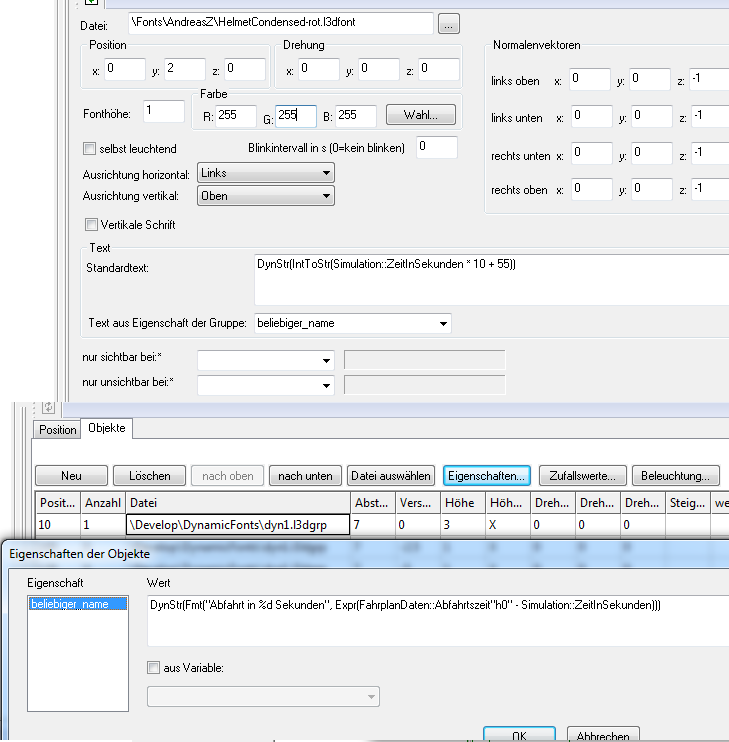
\includegraphics[width=1.0\textwidth]{editor/images/dynamische_schrift.png}
\caption{Möglichkeiten dynamische Schriften zu setzen (oben Gruppenobjekt, unten Streckeneditor)}
\label{fig:editor:dynstr}
\end{figure}

Mit dynamischen Schrifte ist es möglich, den Inhalt von Fonts dynamisch
oder anhand statischer Variablen zu steuern.

Die Ausdrücke können dabei als Standardtext bei Fonts in Gruppenobjekten
eingestellt werden. Oder man setzt den entsprechenden Ausdruck im
Streckeneditor über die Eigenschaften des Objekts.

Dynamische Schriften haben immer die Form \texttt{DynStr()}. Abbildung \ref{fig:editor:dynstr} zeigt zwei Beispiele für die Möglichkeiten Dynamischen Schriften zu definieren.

\subsection{Syntax in EBNF}

Eine Beschreibung der EBNF ist in der \href{http://de.wikipedia.org/wiki/EBNF}{Wikipedia} verfügbar.

\begin{longtable}[c]{@{}lll@{}}
\hline\noalign{\medskip}
\begin{minipage}[t]{0.22\columnwidth}\raggedright
dyn\_font\_expr
\end{minipage} & \begin{minipage}[t]{0.06\columnwidth}\raggedright
=
\end{minipage} & \begin{minipage}[t]{0.73\columnwidth}\raggedright
'DynStr(', func, ')';
\end{minipage}
\\\noalign{\medskip}
\begin{minipage}[t]{0.17\columnwidth}\raggedright
func
\end{minipage} & \begin{minipage}[t]{0.06\columnwidth}\raggedright
=
\end{minipage} & \begin{minipage}[t]{0.78\columnwidth}\raggedright
strarg \textbar{} strfmt \textbar{} expr;
\end{minipage}
\\\noalign{\medskip}
\begin{minipage}[t]{0.17\columnwidth}\raggedright
strarg
\end{minipage} & \begin{minipage}[t]{0.06\columnwidth}\raggedright
=
\end{minipage} & \begin{minipage}[t]{0.78\columnwidth}\raggedright
'FahrplanVars::', var\_chars \textbar{} 'WetterVars::', var\_chars
\textbar{} 'FahrplanDaten::NextHalt("', halt\_chars, '")' \textbar{} 'FahrplanDaten::LastHalt' \textbar{} 'Str::', var\_chars;
\end{minipage}
\\\noalign{\medskip}
\begin{minipage}[t]{0.17\columnwidth}\raggedright
strfmt
\end{minipage} & \begin{minipage}[t]{0.06\columnwidth}\raggedright
=
\end{minipage} & \begin{minipage}[t]{0.78\columnwidth}\raggedright
'Fmt('", fmt\_chars, '",' func\_args, ')';
\end{minipage}
\\\noalign{\medskip}
\begin{minipage}[t]{0.17\columnwidth}\raggedright
func\_args
\end{minipage} & \begin{minipage}[t]{0.06\columnwidth}\raggedright
=
\end{minipage} & \begin{minipage}[t]{0.78\columnwidth}\raggedright
func\_args, ',' , func \textbar{} func;
\end{minipage}
\\\noalign{\medskip}
\begin{minipage}[t]{0.17\columnwidth}\raggedright
expr
\end{minipage} & \begin{minipage}[t]{0.06\columnwidth}\raggedright
=
\end{minipage} & \begin{minipage}[t]{0.78\columnwidth}\raggedright
'Expr(', logic\_expr , ')';
\end{minipage}
\\\noalign{\medskip}
\begin{minipage}[t]{0.17\columnwidth}\raggedright
logic\_expr
\end{minipage} & \begin{minipage}[t]{0.06\columnwidth}\raggedright
=
\end{minipage} & \begin{minipage}[t]{0.78\columnwidth}\raggedright
Ausdruck dynamische Sichtbarkeitssteuerung
\end{minipage}
\\\noalign{\medskip}
\begin{minipage}[t]{0.17\columnwidth}\raggedright
var\_chars
\end{minipage} & \begin{minipage}[t]{0.06\columnwidth}\raggedright
=
\end{minipage} & \begin{minipage}[t]{0.78\columnwidth}\raggedright
Gültiger Variablennamen
\end{minipage}
\\\noalign{\medskip}
\begin{minipage}[t]{0.17\columnwidth}\raggedright
fmt\_chars
\end{minipage} & \begin{minipage}[t]{0.06\columnwidth}\raggedright
=
\end{minipage} & \begin{minipage}[t]{0.78\columnwidth}\raggedright
Gültiger printf Format-String
\end{minipage}
\\\noalign{\medskip}
\begin{minipage}[t]{0.17\columnwidth}\raggedright
halt\_chars
\end{minipage} & \begin{minipage}[t]{0.06\columnwidth}\raggedright
=
\end{minipage} & \begin{minipage}[t]{0.78\columnwidth}\raggedright
Gültiger Haltname, Etwaige Anführungszeichen '' im Haltnamen müssen durch \textbackslash{}'' ersetzt werden
\end{minipage}
\\\noalign{\medskip}
\hline
\noalign{\medskip}
\caption{Syntax der Dynamischen Schriften in EBNF}
\end{longtable}

\subsection{Erklärung}

Die einfachsten dynamischen Schriften greifen schlicht auf Wetter- oder
Fahrplanvariablen zu. Dies geschieht mit der gleichen Syntax wie in
\hyperref[sec.editor.obj.logischeausdruecke]{Logischen Ausdrücken}.

Möchte man eine Zahl darstellen, kann man dies mittels der \texttt{Expr}
Funktion erledigen. Als Argument kann dieser Funktion jeder gültige
Logische Ausdruck übergeben werden. Das numerische Ergebnis des
logischen Ausdrucks, wird in einen String im Dezimalsystem umgewandelt.

Die komplexeste Art von dynamischen Schriften beinhalten den Aufruf der
Funktion \texttt{Fmt}. Diese ermöglicht es, einen komplexen
Ergebnisstring zu erstellen. Als erstes Argument muss dieser Funktion
ein Format-String übergeben werden, welcher bestimmt wie das Ergebnis
zusammengesetzt wird. Dabei können die \href{http://en.wikipedia.org/wiki/Printf#Format_placeholders}{Formatierungsoptionen
von printf} verwendet werden. Danach werden die Argumente für die
Formatierungsplatzhalter übergeben. Es kann hier entweder ein Zugriff
auf eine Variable erfolgen, ein logischer Ausdruck in der Form
\texttt{Expr()} angegeben werden oder wiederum eine Fmt Funktion
verwendet werden.

Zur Verdeutlichung einige Bespiele für mögliche Formatanweisungen.
Leerzeichen wurden dabei durch \emph{␣} ersetzt. Es wird angenommen,
dass \emph{FahrplanVars::h} im Fahrplan als \emph{halt} definiert ist.

\label{sec:editor-obj-dynstr-params}
Ähnlich wie bei der Sichtbarkeitssteuerung können in dynamischen Schriften Variablen in der Form \emph{Str::xxx} verwendet werden. Diese können dann über die Objekteigenschaften im Streckeneditor gesetzt werden. Beim Setzen solcher Eigenschaften kann entweder eine fixe Zeichenkette oder wiederum eine dynamische Schrift in der Form \emph{DynStr(...)} verwendet werden. Wird die Variable in einem verschachtelten logischen Ausdruck verwendet, können die Eigenschaften in der gleichen Art wie bei der Sichtbarkeitssteuerung gesetzt werden.\abversion{2.9}

\begin{longtable}[c]{@{}ll@{}}
\hline\noalign{\medskip}
\begin{minipage}[b]{0.67\columnwidth}\raggedright
Ausdruck
\end{minipage} & \begin{minipage}[b]{0.33\columnwidth}\raggedright
Ergebnis
\end{minipage}
\\\noalign{\medskip}
\hline\noalign{\medskip}
\begin{minipage}[t]{0.67\columnwidth}\raggedright
DynStr(Fmt(''aa\%daa'', Expr(10)))
\end{minipage} & \begin{minipage}[t]{0.33\columnwidth}\raggedright
aa10aa
\end{minipage}
\\\noalign{\medskip}
\begin{minipage}[t]{0.67\columnwidth}\raggedright
DynStr(Fmt(''aa\%4daa'', Expr(10)))
\end{minipage} & \begin{minipage}[t]{0.33\columnwidth}\raggedright
aa␣␣10aa
\end{minipage}
\\\noalign{\medskip}
\begin{minipage}[t]{0.67\columnwidth}\raggedright
DynStr(Fmt(''aa\%4daa'', Expr(1000)))
\end{minipage} & \begin{minipage}[t]{0.33\columnwidth}\raggedright
aa1000aa
\end{minipage}
\\\noalign{\medskip}
\begin{minipage}[t]{0.67\columnwidth}\raggedright
DynStr(Fmt(''aa\%-4daa'', Expr(1)))
\end{minipage} & \begin{minipage}[t]{0.33\columnwidth}\raggedright
aa1␣␣␣aa
\end{minipage}
\\\noalign{\medskip}
\begin{minipage}[t]{0.67\columnwidth}\raggedright
DynStr(Fmt(''aa\%-4daa'', Expr(1234)))
\end{minipage} & \begin{minipage}[t]{0.33\columnwidth}\raggedright
aa1234aa
\end{minipage}
\\\noalign{\medskip}
\begin{minipage}[t]{0.67\columnwidth}\raggedright
DynStr(Fmt(''aa\%04daa'', Expr(2)))
\end{minipage} & \begin{minipage}[t]{0.33\columnwidth}\raggedright
aa0002aa
\end{minipage}
\\\noalign{\medskip}
\begin{minipage}[t]{0.67\columnwidth}\raggedright
DynStr(Fmt(''aa\%04daa'', Expr(11111)))
\end{minipage} & \begin{minipage}[t]{0.33\columnwidth}\raggedright
aa11111aa
\end{minipage}
\\\noalign{\medskip}
\begin{minipage}[t]{0.67\columnwidth}\raggedright
DynStr(Fmt(''aa\%-10saa'', FahrplanVars::h))
\end{minipage} & \begin{minipage}[t]{0.33\columnwidth}\raggedright
aahalt␣␣␣␣␣␣aa
\end{minipage}
\\\noalign{\medskip}
\begin{minipage}[t]{0.67\columnwidth}\raggedright
DynStr(Fmt(''aa\%8saa'', FahrplanVars::h))
\end{minipage} & \begin{minipage}[t]{0.33\columnwidth}\raggedright
aa␣␣␣␣haltaa
\end{minipage}
\\\noalign{\medskip}
\hline
\noalign{\medskip}
\caption{Beispiele für Formatanweisungen}
\end{longtable}

\texttt{FahrplanDaten::NextHalt("")} liefert den nächsten Halt
\emph{nach} halt. Kommt in halt ein Anführungszeichen '' vor, muss dieses durch \textbackslash{}'' ersetzt werden.

\texttt{FahrplanDaten::LastHalt} liefert den letzten Halt der keine Betriebsstelle ist

\subsection{Performance}

Schriften die sich sehr oft ändern, sollten mit Bedacht eingesetzt
werden, da sie die fps relativ stark beeinflussen.

Verwendet eine Schrift nur konstante Werte (FahrplanVars oder konstante
logische Ausdrücke) so hat diese kaum einen Einfluss auf die Performance

\subsection{Beispiele}

\begin{verbatim}
DynStr(Fmt("Abfahrt in %d Minuten",
    Expr((Funktionen::TimeDif(
    FahrplanDaten::Abfahrtszeit("h0"), 
    Simulation::ZeitInSekunden)) / 60))
\end{verbatim}

\begin{verbatim}
DynStr(Fmt("%02d:%02d:%02d", 
    Expr(Simulation::ZeitInSekunden / 60 / 60),
    Expr(Simulation::ZeitInSekunden / 60 % 60), 
    Expr(Simulation::ZeitInSekunden % 60)))
\end{verbatim}

\begin{verbatim}
DynStr(IntToStr(Simulation::ZeitInSekunden * 10))
\end{verbatim}

\begin{verbatim}
DynStr(FahrplanVars::Zugziel)
\end{verbatim}

\chapter{Strecken}
\section{Gleis}
\label{sec.editor.gleis}

\subsection{Gleiseigenschaften}
\label{subsec.editor.gleis.gleiseigenschaften.signal}

\subsubsection{Signal}
\label{subsubsec.editor.gleis.gleiseigenschaften.signal}

\input{editor/Strecke/OptionGruppensignal.tex}
\subsubsection{Signaloptionen}
\label{subsubsec.editor.gleis.gleiseigenschaften.signaloptionen}

\paragraph{Gleisabhängiges Zusatzsignal}
Diese Funktion kann für Zusatzsignale benutzt werden, die je nach Gleis ein bestimmtes Font anzeigen sollen, ähnlich dem Zs2. Bei diesem Zusatzsignal wird aber auf der KBS-Strecke in Fahrrichtung rückwärts nach einem Eintrag für dieses Zusatzsignal gesucht. Mit dem Setzen eines Referenzzeichens (Buchstabe, Zahl) kann der entsprechende Font angesteuert werden. Es wird ab Signal maximal 1000 m rückwärts nach der Zusatzsignalreferenz gesucht.

Einrichten eines solchen Zusatzsignals:
\begin{itemize}
\item
In einem Gruppenobjekt den entsprechenden Schriftzug wählen und beim Popup-Menu  "Text aus Eigenschaft der Gruppe" den Eintrag "GlAbhZSig" auswählen.
\item
In den Eigenschaften einer Strecke an der gewünschten Position eine neue Signaloption definieren und bei "Gleisabhängiges Zusatzsignal" das Häckchen setzen. Beim Eintrag Referenzzeichen ein Zeichen (Buchstabe, Zahl) eintragen, das dem gewünschten Fontzeichen entspricht.
\end{itemize}
\label{sec:editor-obj}
Bis zur Version 2.8.3 war das Objektsystem des Loksims relativ einfach unterteilt: Sämtliche 3D-Objekte waren entweder einfache Objekte (.l3dobj) oder Gruppenobjekte (.l3dgrp), wobei Gruppenobjekte aus beliebig vielen Objekten (.l3dobj) und Schriften bestehen konnten.

Ab Version 2.9 ist das System flexibler gestaltet: Wie bisher sind einfache .l3dobj Objekte und Gruppenobjekte .l3dgrp die ''Eckpfeiler'' des Objektsystems. Jedoch können Gruppenobjekte nun aus beliebigen Objekte die von Loksim unterstützt werden bestehen. Dies heißt, Gruppenobjekte können wiederum andere Gruppenobjekte beinhalten und auch \hyperref[sec:editor-obj-externe]{Objekte in externen Dateiformaten}.


\section{Objekte}
\label{sec:editor-obj-l3dobj}
Objekte (.l3dobj) sind das Grundgerüst für die 3D-Welt. Objekte bestehen aus Punkten und Flächen.

\subsection{Objekteigenschaften}
\begin{description}
\item[Textur und Transparenz]\hyperref[sec:editor-obj-textur]{nähere Details}
\item[Rückseiten sichtbar] Normalerweise ist eine Fläche immer nur von einer Seite sichtbar, wobei die sichtbare Seite anhand der Reihenfolge der Punkte einer Fläche abhängig ist. Wird diese Option gesetzt, sind alle Flächen von beiden Seiten sichtbar. Diese Option sollte nur bei kleinen oder selbstleuchtenden Objekten gesetzt werden, normalerweise sollte explizit eine Rückseite mittels zweiter Fläche eingefügt werden. Nur so ist eine ordentliche Beleuchtung von beiden Seiten möglich
\item[selbst leuchtend] Wird diese Option gewählt wird das Objekt nicht durch das Beleuchtungssystem beleuchtet, dadurch gibt sich ein Effekt als würde das Objekt selbst leuchten. Normalenvektoren sind bei selbst leuchtenden Objekten nicht relevant
\item[Objekt dreht mit dem Betrachter mit] Wird diese Option gesetzt, dreht sich das Objekt immer so, dass die Vorderseite zum Betrachter zeigt. So können flache Objekte aus gewisser Entfernung wie plastische Objekte wirken. 
\item[Normalenvektor pro Fläche] Ist diese Option gewählt, werden die Normalenvektoren nicht wie sonst pro Punkt eingegeben, sondern pro Fläche (\hyperref[sec:editor-obj-l3dobj-normalen]{nähere Details})\abversion{2.9}
\end{description}


\subsection{Punkte}
Jeder Punkt hat eine bestimmte Position im Raum und kann einen Normalenvektor enthalten.

\subsection{Flächen}\abversion{2.9}
\label{sec:editor-obj-l3dobj-flaeche}
Flächen bestehen aus drei oder mehr Punkten in \emph{einer Ebene}. Bei der Definition einer Fläche dürfen keine Löcher entstehen. Mit eine Rechtsklick auf eine Fläche kann automatisch die Rückseite zu der gewählten Fläche eingefügt werden.

\subsection{Normalenvektoren}\abversion{2.9}
\label{sec:editor-obj-l3dobj-normalen}
Normalenvektoren werden zur Beleuchtung von Objekten verwendet. Bei ''eckigen Oberflächen'' sollten die Normalenvektoren immer \emph{senkrecht} auf die Fläche stehen. Bei ''runden Oberflächen'' kann durch die richtige Wahl der Normalenvektoren der Eindruck der runden Oberfläche verbessert werden. Diese Anleitung kann keine genaue Einführung in Normalenvektoren geben, erfahrene Objektbauer können aber an vielen Stellen im Internet genauere Details dazu finden. Normalenvektoren sind kein Konzept des Loksims, sondern werden  generell in der 3D-Modellierung und -Darstellung genutzt.

Da Loksim bisher recht gut mit komplett falsch gesetzten Normalenvektoren umgegangen ist, hat sich beim Loksim-Objektbau eine gewisse Schlampigkeit bzgl. Normalenvektoren entwickelt. Ab Version 2.9 gibt es deshalb eine gravierende Änderung: Standardmäßig wird bei Objekten die Option \emph{Normalenvektor pro Fläche} gesetzt. Wird diese Option verwendet, kann es keine unterschiedlichen Normalenvektoren pro Fläche geben. Außerdem steht über das Menü - Bearbeiten die Funktion \emph{Normalenvektoren automatisch berechnen} zur Verfügung. Diese erzeugt Normalenvektoren die senkrecht auf die jeweilige Fläche stehen. Für die meisten Objekte sollte diese Option ausreichen. Für runde Objekte muss diese Einstellung jedoch deaktiviert werden und die Normalenvektoren wie bisher pro Punkt definiert werden.

Da Loksim in Zukunft ein verbessertes Beleuchtungssystem bekommen wird, gibt es folgende Regelung: Bei Objekten die mit Version 2.9 oder neuer erstellt oder abgeändert wurden wird angenommen, dass sie mit korrekten Normalenvektoren ausgestattet sind. Ältere Objekte werden vorraussichtlich anders verarbeitet werden, sodass falsche Normalenvektoren nicht so sehr ins Gewicht fallen.

\subsection{Zoomen/Verschieben}\abversion{2.9}
\label{sec:editor-obj-l3dobj-punkteverschieben}
Über das Bearbeiten Menü stehen die Funktionen \emph{Punkte verschieben/zoomen} und \emph{Objekt am Nullpunkt zentrieren} zur Verfügung. Bei erster kann gewählt werden welche Punkte verschoben/gezoomt werden sollen und um welchen Wert die Änderung erfolgen soll. Bei zweiter Funktion wird automatisch der Nullpunkt des Objekts berechnet und der Dialog zum Verschieben aller Punkte geöffnet. Hier sind bereits die Werte eingetragen welche nötig sind, um das Objekt in den Nullpunkt zu verschieben. Die Werte können vor dem Verschieben noch angepasst werden.

\section{Gruppenobjekte}\abversion{2.9}
\label{sec:editor-obj-grp}
Gruppenobjekte können beliebige andere von Loksim unterstützte Objekte enthalten. Für jedes Objekt kann die Position, Rotation und Skalierung für jede Achse eingestellt werden. Außerdem können einzelne Objekte mit der \hyperref[sec:editor-obj-sichtbarkeitssteuerung]{Sichtbarkeitssteuerung} ein- und ausgeblendet werden.

Die 2D-Vorschau unterstützt derzeit nur loksim-eigene Formate, externe Objektformate werden in der 2D-Vorschau nicht angezeigt.
\subsection{Verschieben}\abversion{2.9}
\label{sec:editor-obj-grp-verschieben}
Über das Bearbeiten Menü stehen die Funktionen \emph{Punkte verschieben} und \emph{Objekt am Nullpunkt zentrieren} zur Verfügung. Bei erster kann gewählt werden welche Objekte verschoben werden sollen und um welchen Wert die Änderung erfolgen soll. Bei zweiter Funktion wird automatisch der Nullpunkt des Objekts berechnet und der Dialog zum Verschieben aller Objekte geöffnet. Hier sind bereits die Werte eingetragen welche nötig sind um das Gesamtobjekt in den Nullpunkt zu verschieben. Die Werte können vor dem Verschieben noch angepasst werden.


\section{Externe 3D-Objektmodellformate}\abversion{2.9}
\label{sec:editor-obj-externe}
Es besteht die Möglichkeit alle von Assimp\footnote{\url{http://assimp.sourceforge.net/main_features_formats.html}} unterstützten externe Objektformate zu verwenden. Allerdings ist das Objektsystem immer noch auf .l3dgrp und .l3dobj Dateien ausgerichtet. Alles was also nicht mittels .l3dgrp oder .l3dobj Dateien möglich ist, kann derzeit auch nicht durch externe Formate umgesetzt werden.

Je nach Bedarf der Objektbauer wird die Unterstützung externer Dateiformate noch erweitert werden.

\subsection{Konvertieren externer 3D-Objektmodellformate}
\label{sec:editor-obj-externe-konvertieren}
Über die Kommandozeile lassen sich alle unterstützen Dateiformate in Loksim Gruppen(objekte) umwandeln. Dafür muss der LoksimEdit in der Konsole folgenderweise aufgerufen werden:
\begin{verbatim}
LoksimEdit -convert <Pfad Quellobjekt> <Pfad Zielobjekt>
\end{verbatim}
Der ''Pfad Zielobjekt'' sollte dabei auf eine nicht existierende Datei in einem \emph{leeren} Ordner verweisen. Beim Konvertieren werden möglicherweise mehrere Dateien erstellt, bestehende Dateien die zufällig den gleichen Namen tragen werden dabei ohne Rückfrage überschrieben.

\section{Gleise}
\label{sec:editor-gleise}
Gleise sind spezielle - von Loksim selbst erzeugte - Objekte. Das Aussehen der Gleise wird mittels .l3drail Dateien beschrieben.

\begin{description}
\item[Transparenz] Wie bei herkömmlichen Objekten können auch Gleise teilweise transparent sein. Nähere Details dazu findet man im Abschnitt über \hyperref[sec:editor-obj-transparenz]{Transparenz bei Objekten}\abversion{2.9.3}
\item[Normalenvektoren senkrecht] Bis Version 2.9.2 wurden sömtliche Normalenvektor bei den generierten Gleise auf 0/1/0 gestellt. Wird die Option ''Normalenvektoren senkrecht'' aktiviert, werden die Normalenvektoren korrekt berechnet und stehen immer senkrecht zur jeweiligen Fläche.\abversion{2.9.3}
\item[Keine 3D-Darstellung] Ein beliebter Trick für die Landschaftdarstellung und Objektpositionierung ist das Anlegen unsichtbarer Gleise. Wird diese Option gewählt ist dies ein Hinweis für das Programm, dass entsprechende Gleise nicht für die Darstellung in 3D verwendet werden, sondern nur Hilfsgleise für Objekte bzw. Landschaft sind. Dies führt zur Reduzierung von Ladezeiten und Verbesserung der fps\abversion{2.9.3}
\end{description}

			
\chapter{Loks}
\section{Führerstand}
\label{sect.editor.lok.fst}
Loksim unterstützt derzeit nur 2D-Führerstände. Der Füherstand besteht aus einer einzelnen Textur auf welche die Instrumente und Schalter gezeichnet werden
\begin{description}
\item[Bitmap] Führerstandsbild
\item[Bitmap Nacht] Führerstandsbild, welches in der Nacht bzw. bei Dunkelheit angezeigt wird. Tag- und Nachtführerstandsbild werden dabei linear überblendet um einen fließenden Übergang zu erreichen. Dafür wird im Normalfall die aktuelle (Wetter)helligkeit herangezogen. Ist in der Strecke jedoch eine spezielle Beleuchtung des Gleises eingetragen, werden diese Beleuchtungseinstellungen verwendet.\\
Es ist zu beachten, dass sich die Instrumente bei Nacht- und Tagführerstand exakt an den gleichen Positionen befinden müssen und die Bitmaps exakt gleich groß sein müssen. Außerdem muss die gleiche Transparenzfarbe verwendet werden bzw. bei beiden Bitmaps der Alphakanal verwendet werden.\abversion{2.8.3}
\item[Streckenfenster] Hier müssen die Koordinaten bzw. die Größe des Streckenfensters eingetragen werden. In diesem Bereich wird die 3D-Landschaft hineingezeichnet.
\item[Transparentfarbe] Falls \emph{Transparenz aus Alphakanal} nicht gewählt wird, werden alle Pixel welche die hier angegebene Farbe besitzen vollständig transparent dargestellt.
\item[Transparenz aus Alphakanal] Wird diese Option gewählt, wird die Transparenz aus dem Alphakanal des Bitmaps genommen. Damit können auch halbtransparente Bereiche definiert werden.\abversion{2.8.3}
\item[Auflösung] Größe des Führerstandsbild
\end{description}
\section{Dialog Motor (Antriebsdaten)}
Wenn im Folgenden von Motor die Rede ist, so ist das Antriebskonzept im Loksim gemeint. Es wird immer mit den Summen aller Motoren eines Triebfahrzeuges gerechnet. Loksim kennt derzeit keine Differenzierung einzelner Motoren, Motortypen oder Triebfahrzeugarten.

Die nachstehenden Angaben sind zwingend notwendig, damit Loksim mit seinem Antriebsmodell rechnen kann. Leider sind sie nicht immer leicht herauszufinden. Am meisten Infos findet man in den Handbüchern zu den Triebfahrzeugen, wenn dies nicht möglich ist, vielleicht mit einer Suche im Internet.

\subsection{maximale Geschwindigkeit (km/h)}
Wird zur Berechnung des Motorwiderstandes benötigt.
Ist gewöhnlich bei jeder Lok irgendwo angeschrieben.

\subsection{maximale Motorspannung (V)}
Wird benötigt zur Berechnung des Motorwiderstandes sowie der je nach Fahrstufe am Motor anliegenden Spannung.
Dieser Wert dürfte meist nur Fachleuten bekannt sein. Allgemein kann man sagen, dass er sich im Bereich von 400-700 Volt bewegt mit einem mittleren Wert bei ca. 500-550 Volt. Vor allem moderne Motoren arbeiten aber auch mit Spannungen bis über 1 kV.

\subsection{Wirkungsgrad der Motoren (\%)}
Verwendung siehe maximale Lokleistung.
Noch ein Wert, der wohl nicht mal immer den Fachleuten bekannt ist. Allgemein zwischen 80 – 95 \%.
Mit diesem Wert werden alle Verluste repräsentiert, die anfallen zwischen der Leistung, die in die Motoren gesteckt wird und der Leistung, die am Rad zur Verfügung steht.

\subsection{maximale Lokleistung (kW)}
Es handelt sich um die mechanische Leistung, die am Rad anliegt. Bei der Berechnung des Motorstroms wird im Loksim der Verlust dazugerechnet durch Einbezug des Motor-Wirkungsgrades und mit diesem Strom wird dann die Leistung gerechnet, die in den Motor gesteckt wird.
Dieser Wert dürfte bei neueren Loks (Asynchronmotoren) oft in Erfahrung zu bringen sein, bei älteren Loks sind jedoch meist die Stunden- und Dauerleistung angegeben, welche immer tiefer als die maximale Leistung sind. Wenn die Loks eine Primärstrombegrenzung haben, kann über die Primärleistung $Oberspannung [V] * \frac{Primaerstrom [A]}{1000}$ ebenfalls auf die ungefähre maximale Leistung geschlossen werden. Die \%-Zahlen sind Näherungswerte. Es ist mit einer Streuung von ungefähr +/- 10\% zu rechnen. Der Bezug auf die Primärleistung ist am wenigsten genau.
Die maximale Lokleistung ist
\begin{itemize}
\item ca. 145 \% der Dauerleistung am Rad
\item ca. 135 \% der Dauerleistung an der Motorwelle
\item ca. 135 \% der Stundenleistung am Rad
\item ca. 125 \% der Stundenleistung an der Motorwelle
\item ca.   80 \% der Primärleistung
\end{itemize}
Bei älteren Loks wird noch die alte Einheit PS verwendet. 1 PS entspricht 736 W oder 0.736 kW.

\subsection{Maximaler Motorstrom (A)}
Wird benutzt, um die Fahrleistung zu begrenzen auf die maximal zulässigen Motorstromwerte. 
Ist bei älteren Loks meist irgendwo im Führerstand angeschrieben und in den Handbüchern verzeichnet, bei neueren selten bekannt.
Wird die Loksim-Funktion \emph{Motorstrom berechnen} benutzt, berechnet Loksim den Motorstrom aus max. Leistung und max. Motorspannung. Dies entspricht aber vor allem bei älteren Loks oft nicht dem max. Motorstrom, er ist meist höher.

\subsection{Wirkungsgrad Transformator (\%)}
Verwendung siehe Oberspannung.
Auch diese Angabe ist kaum in Erfahrung zu bringen. Der Wirkungsgrad liegt im Bereich von 90 – 97 \%.

\subsection{Oberspannung (V)}
Aus momentaner Leistung und Wirkungsgrad des Transformators wird der Oberstrom berechnet.
Die benutzte Netzspannung ist wiederum bekannt.

\subsection{maximale Zugkraft (kN)}
Wird unter anderem zur Berechnung der Beschleunigung verwendet.
Dieser Wert dürfte meist irgendwo in der Literatur/Internet zu finden sein.
Bei älteren Loks wird die Zugkraft noch in kg oder kp angegeben. 1 kg oder 1 kp = 9,81 N  oder 0,00981 kN


\subsection{Motorparameter}
Die Erklärungen und Anleitungen zu den Motorparametern gelten vor allem für elektrische Triebfahrzeuge, die mit Stufenschalter oder ähnlich ausgerüstet sind. Für moderne Drehstromloks, Dieselloks mit Gangschaltung und Dampfloks  ist es derzeit nicht möglich, ein vorbildgerechtes Verhalten aufgrund von lokspezifischen Daten einstellen zu können. Trotzdem kann ein annähernd vorbildliches Verhalten durch geschicktes Einstellen der Parameter erreicht werden.

Mit Hilfe der drei Motorparameter wird eine hyperbelähnliche Kurve berechnet, die als Widerstandskurve im Dialog ersichtlich ist und als Basis zur Simulation des Antriebsverhaltens des Triebfahrzeugs dient. Diese Kurve ist typisch für Triebfahrzeuge mit Reihenschlussmotoren (auch Serie- oder Universalmotoren genannt). Diese Motoren wurden verwendet bis zum Aufkommen moderner Loks mit Asynchron-Drehstrommotoren, die eine andere Kennlinie besitzen.

Zur Veranschaulichung, wie die drei Parameter (am Beispiel der Ae 610 der SBB) eingestellt werden, siehe \fref{fig:editor:motorparameter}

\begin{figure}
\centering
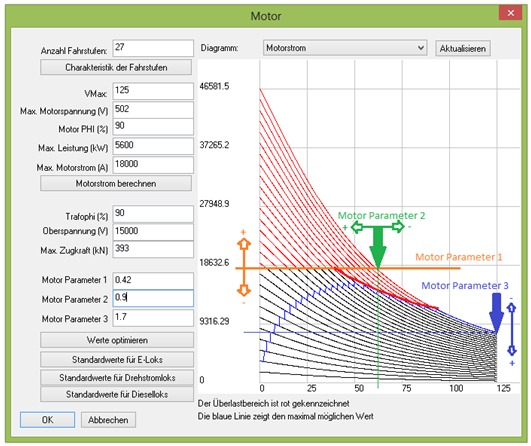
\includegraphics[width=1.0\textwidth]{editor/images/motorparameter.png}
\caption{Motorparameter der Ae 610 der SBB}
\label{fig:editor:motorparameter}
\end{figure}

\subsubsection{Motorparameter 1 (orange)}
Dient zur Festlegung der Stufe (oder Punkt zwischen zwei Stufen), bei der der maximale Motorstrom erreicht wird. (Im Beispiel unten zwischen der 10. und 11. Stufe).
Dazu ganz links bei Geschwindigkeit 0 aufsteigend die Anzahl schwarzer Linien zählen. Parameter 1 so lange verändern, bis gewünschte Stufe erreicht wird.

\subsubsection{Motorparameter 2 (grün)}
Legt fest, ab welchem Punkt der Motorstrom auf der höchsten Fahrstufe in Bezug auf eine bestimmte Geschwindigkeit zu sinken beginnt.
Durch Verändern des Parameters 2 kann der Punkt, an dem sich die waagrechte Linie des max. Motorstroms und die Linie der höchsten Stufe kreuzen, so waagrecht verschoben werden, bis die Senkrechte durch diesen Punkt unten auf der Geschwindigkeitsskala auf die gewünschte Geschwindigkeit trifft.

\subsubsection{Motorparameter 3 (blau)}
Bestimmt den Motorstrom, der bei maximaler Geschwindigkeit auf der höchsten Fahrstufe noch fließt.
Mit dem Verändern des Parameters 3 kann die Höhe des Motorstroms eingestellt werden, der bei max. Geschwindigkeit noch fliesst.

Es ist zu beachten, dass sich die Motorparameter 2 und 3 gegenseitig beeinflussen. Es ist deshalb meist nötig, den nicht veränderten Parameter etwas nachzuregeln, bis die Kennlinien mit dem Vorbild übereinstimmen.

Auf \fref{fig:editor:motorparameter} wurde die Oberstrom- (oder Primärstrom-)begrenzung durch eine rote Linie gekennzeichnet. Bei Loks, die keine Oberstrombegrenzung haben, fällt diese "Delle" weg.


\subsubsection{Werte optimieren}
Wenn detaillierte Werte einer Lok bekannt sind, kann man diese in eine Tabelle eingeben und Loksim erstellt daraus eine Widerstandskurve, indem es selbst die drei Parameter berechnet.

\subsection{Standardwerte für E-Loks, Drehstromloks und Dieselloks}
Stehen keine genauen Angaben für eine Lok zur Verfügung, kann man mit dieser Funktion die Kennlinien durch Loksim erstellen lassen. Ebenso dient sie als Ausgangsbasis und der Ersteller des Führerstandes kann durch Veränderung der Motorparameter die Kennlinien nachträglich manuell nach seinen Wünschen einstellen (siehe oben).

\subsubsection{Drehstromloks}
Der Parameter 1 hat bei diesen Loks eigentlich keine Bedeutung, denn hier wird mit dem Fahrhebel die prozentuale Zugkraft eingestellt. Die „Stufenlinien“ müssten daher eigentlich waagrecht liegen. Loksim ist aber zur Zeit noch nicht für Drehstromloks optimiert.
Immerhin kann mit dem Parameter 1 der Punkt mitbeeinflusst werden, an dem die maximale Lokleistung zur Verfügung steht (siehe auch Parameter 2).

Annäherungsweise kann der Parameter 2 so eingestellt werden, dass die maximale Leistung bei der Geschwindigkeit erreicht wird, bei der die Zugkraft zu sinken beginnt.

Ebenso kann mit dem Parameter 3 der Punkt angesteuert werden, an dem noch eine bestimmte Zugkraft bei max. Geschwindigkeit erbracht wird.

\subsubsection{Dieselloks}
Wenn es sich um Diesel-Generator-Loks handelt, kann die Lok wie eine Stufenschalterlok eingestellt werden. Die Dieselthematik ist zur Zeit im Loksim noch nicht umgesetzt.

\subsubsection{Dampfloks}
Da die Dampfloks ein sehr ähnliches Verhalten wie Stufenschalterloks haben, kann ihr Verhalten mittels der drei Parameter ziemlich vorbildlich nachgebaut werden, allerdings mit „artfremden“ Parametern (Spannung, Strom). Die Dampfthematik ist derzeit im Loksim noch nicht umgesetzt.

\subsection{Diagramm}
Mit dem Popup-Menu kann zwischen den Ansichten Leistung, Oberstrom, Motorstrom,  Motorspannung, Widerstand und Zugkraft gewählt werden.

\subsection{Bemerkung}
Die Zugkraft ist mit einem Fehler behaftet, was sich insbesondere bei Drehstromloks mit Zugfahrkrafthebeln bemerkbar macht. Das Antriebsmodell des Loksim wird derzeit überarbeitet (inklusive Bremsen) und voraussichtlich in einer der nächsten Versionen veröffentlicht.

\section{Indusi/PZB}

In Version 2.8.2 wurde eine Überarbeitung der PZB90 eingebaut. Dieser
Abschnitt bezieht sich derzeit, nur auf die PZB-Versionen, welche von
dieser Überarbeitung betroffen sind.

\subsection{Art der Indusi}

Folgende PZB-Arten wurden mit Version 2.8.2 erneuert:

\begin{itemize}
\itemsep1pt\parskip0pt\parsep0pt
\item
  PZB90 I60R
\item
  PZB90 I60/ER24
\item
  PZB90 PZ80R
\item
  PZB90 I80
\end{itemize}

Die PZB Version kann für diese Typen im \hyperref[sec.editor.pzb.einstellungen]{PZB Einstellungsdialog} geändert
werden

Eine detaillierte Beschreibung der Systeme kann im \href{http://www.dbnetze.com/regelwerke}{betrieblich-technischen Regelwerk der DB Netz AG}
nachgelesen werden.

Bei I60R ertönt der Sound für die Freitaste nur, wenn tatsächlich eine
Befreiung möglich ist. Bei I60/ER24 ertönt dieser Sound immer wenn die
Freitaste gedrückt ist.

Kontrolllauf und PZ80R Kontrollschalter sind derzeit nicht implementiert.

Jene Optionen die mit \emph{(veraltet)} gekennzeichnet sind, sollten bei
neuen Loks nicht mehr verwendet werden. Diese Optionen stehen nur
aufgrund Rückwärtskompatiblität zu älteren Führerständen zur Verfügung

\subsection{Sounds}

\begin{description}
\item[Indusihupe (WT, FT)]
Sound welcher bei Betätigung von Wachsamkeitstaste bzw. Freitaste
abgespielt wird. Dieser wird in einer Schleife abgespielt, solange die
entsprechende Taste gedrückt ist.
\item[Indusibefehl]
Sound welcher in einer Schleife abgespielt wird, solange die
Befehlstaste aktiv ist.
\item[Zwangsbr.-Indusi]
Dieser Sound wird in einer Schleife während einer Zwangsbremsung
abgespielt.
\item[Zwangsbr.-Indusi nur einmal]
Dieser Sound wird exakt einmal am Anfang einer Zwangsbremsung
abgespielt.
\item[Ende 500Hz Überwachung]
Sound wird am Ende einer 500Hz Überwachung abgespielt, falls sie im
restriktiven Modus endet.
\item[Überschreiten V-Pruef]
Dieser Sound wird beim Überschreiten der PZB-Prüfgeschwindigkeit
wiederholt abgespielt. Je nach PZB-Art kommt dieser Sound sofort bei
Überschreiten oder erst nach einer definierten Zeitspanne.
\end{description}

\subsection{Leuchtmelder und Anzeigen}

Die Leuchtmelder und Anzeigen werden wie andere Anzeigen im Lokeditor
definiert. Bei Einsatz von PZ80R sollte von den Leuchtmeldern nur der
Leuchtmelder Indusi 95 (LVZ grün) definiert werden, aber dafür die
Anzeige IndusiVZiel. Bei den anderen Arten sollte alle Leuchtmelder
gesetzt werden, jedoch die Anzeige IndusiVZiel nicht.

\subsection{PZB Einstellungen}
\label{sec.editor.pzb.einstellungen}

Im Lokeditor ist über das Menü Bearbeiten - PZB Einstellungen ein Dialog
abrufbar, der weitere Einstellungen für die PZB ermöglicht.

Zum Großteil geht es hier um Eigenschaften der PZB die nicht exakt aus
den uns zur Verfügung stehenden Unterlagen implementiert werden konnten
oder wo es in der Praxis konträre Erfahrungen gibt. Jedoch gibt es auch
Einstellungen die bekanntermaßen von Lok zu Lok unterschiedlich sind

\begin{description}
\item[Version]
Hier kann die Version der PZB90 ausgewählt werden. Es stehen alle
Versionen die in der Realität vewendet werden und wurden (1.5, 1.6 und
2.0) zur Verfügung
\item[Befehlstaste ist ein Schalter]
Ein Druck auf die Befehlstaste aktiviert die Befehlstaste und ein
zweiter Druck deaktiviert diese.
\item[Befehlstaste ist ein Taster]
Befehlstaste ist nur aktiv, solange die Taste gedrückt wird. Dies ist
meist bei neueren Tfz der Fall.
\item[Zeit für Wachsamkeitstaste]
Definiert die Zeit in Millisekunden innerhalb welcher nach einer 1000Hz
Beeinflussung die Wachsamkeitstaste gedrückt werden muss. Normalerweise
sind dies 4 Sekunden, im Fall der MVB jedoch 2,5 Sekunden.
\item[Befreiung aus Zwangsbremsung...]
Annahme: Bei Stillstand nach einer Zwangsbremsung aufrund einer 1000Hz
Überwachung sind bereits 700m oder mehr ab Beginn der Beeinflussung
vergangen. Nun muss die Freitaste zur Befreiung aus der ZB betätigt
werden.

Falls die Option kann gleichzeitig Befreiung aus 1000Hz Überwachung
bewirken gesetzt ist, bewirkt ein Druck auf die Freitaste die Befreiung
aus der ZB, sowie die Befreiung aus der 1000Hz Überwachung.

Ist hingegen bewirkt niemals gleichzeitig Befreiung aus einer
Überwachung gewählt, bewirkt ein Drücken der Freitaste ausschließlich
die Befreiung aus der ZB.
\item[Dauerbetätigung PZB Tasten]
Wird hier eine Option gesetzt, wird die entsprechende Taste nach der
bestimmten Zeit und/oder Entfernung unwirksam. 0 bedeutet, dass die
Taste kein Zeit- bzw. Entfernungsmaximum besitzt.

Die Richtlinien der ÖBB geben eine maximale Distanz von 225m für alle
Tasten an.
\item[Status 'befreit' wird an überlagerte Überwachung weitergegeben]
Wird diese Option gesetzt, wird der Status 'befreit' einer 1000Hz
Überwachung an eine überlagerte 1000Hz Überwachung weitergegeben.
Angenommen folgende Situation: 0m/1000Hz, 800m/Befreiung, 1000m/1000Hz,
1400m/500Hz: Ist diese Option nicht gesetzt, erfolgt am 500Hz Magnet
keine Zwangsbremsung, solange man die entsprechende Geschwindigkeit
einhält. Ist die Option gesetzt, bekommt man am 500Hz Magnet immer eine
ZB aufgrund nicht erlaubter Befreiung
\item[Sonderform]
Über diese Einstellungen können Sonderformen der PZB simuliert werden.

Derzeit ist nur die Sonderform \emph{Stadtbahn} möglich. Bei dieser
Variante gibt es neben dem Wechselblinken ein Gleichblinken, bei welchem
65km/h gefahren werden dürfen.
\end{description}


\section{Türsteuerung}
\begin{description}
\item[mind. Türschliesszeit (Sek)] Geben Sie hier an, wieviele Sekunden die Türen mind. zum Schließen benötigen. Durch div. Einflüsse kann das Schließen auf ggf. zufällig länger dauern.
\item[Deaktiver Türmelder (Gtz)] Geben Sie hier an, welchen Melderzustand bei Güterzugdienst verwendet werden soll. Sie können zwischen Zustand ein bzw. aus wählen.
\item[Türsnd (schliessen)] Geben Sie hier die Sounddatei an, die während des Schließen der Türen abgespielt werden soll. Das Geräusch darf nur ein Dauerton beinhalten.
\item[Türsnd (geschlossen] Geben Sie hier die Sounddatei an, die nach dem Schließen der Türen abgespielt werden soll. Das Geräusch darf nur ein Dauerton beinhalten.
\item[Türsnd (öffnen)] Geben Sie hier die Sounddatei an, die während des Öffnen der Türen abgespielt werden soll.
\end{description}
Für ein optimales Zusammenspiel von Sound und Anzeigen im Führerstand, sollte die \emph{mind. Türschließzeit} der Dauer der wav-Datei \emph{TürSnd (schließen)} entsprechen.

\section{Diverses}
\subsection{Wegmessung / Zuglängenzähler}\abversion{2.8.3}
Der \hyperref[sec.sim.steuerung.diverses.wegmessung]{Zuglängenzähler} besteht im Loksim aus zwei Sounds:
\begin{description}
\item[Sound Wegmessung Beginn] Dieser Sound wird beim Start der Wegmessung abgespielt (optional)
\item[Sound Wegmessung Ende] Dieser Sound wird nachdem eine Zuglänge zurückgelegt wurde abgespielt
\item[Wegmessung aktivierbar ab x km/h] Falls diese Einstellung auf einen Wert größer als 0 eingestellt ist, lässt sich die Wegmessung erst ab der eingestellten Geschwindigkeit starten und nicht im Stillstand
\end{description}

\chapter{Wettereditor}
\section{Niederschlag}

Ab Version 2.8.2 besteht in Wetterdateien die Möglichkeit den Schneefall
zu steuern.

\emph{Die Umsetzung des Niederschlags im Loksim ist derzeit auf keinen
Fall ausgereift und sieht nicht in allen Situationen wirklich gut aus.
Er wurde ursprünglich als "Weihnachtsüberraschung" eingebaut und noch
nicht vollständig umgesetzt.}

Schneefall kann im Wettereditor pro Zeitbereich mit der Checkbox
Schneefall aktiviert werden


\chapter{Allgemeines}
\section{Dateien überschreiben}\abversion{2.9}
\label{sec:editor-allg-dateienueberschreiben}

Im Gegensatz zu vielen anderen (3D-)Anwendungen verwendet Loksim ein vollkommen offenes Dateiformat für sämtliche Addons. Zusätzlich sind Dateien nicht speziell an ein Package gebunden, sondern jedes einzelne Objekt, Textur, Führerstand, etc. kann im LoksimEdit geöffnet, betrachtet und sogar geändert werden.

Je nach \emph{Lizenz des Package} und der darin verwendeten Teile können Teile eines anderen Package auch - eventuell sogar in einer abgeänderten Form - in einem eigenen Package wiederverwendet werden. 

Bei einer Änderung einer fremden Datei ist jedoch \emph{immer eine Kopie anzulegen}, fremde Dateien dürfen \emph{niemals überschrieben} werden.

Lange Zeit wurde diese essentielle Übereinkunft technisch überhaupt nicht überprüft und nur eine sorgfältige Verwendung des LoksimEdit hat vor unabsichtlichem Überschreiben fremder Dateien geschützt. Mit Version 2.9 wurde hierfür zusätzlich eine technische Unterstützung eingführt, die das unabsichtliche Überschreiben fremder Dateien verhindern soll. Die Implementierung basiert dabei auf folgenden Grundsätzen:
\begin{itemize}
\item Jede Datei besitzt einen oder mehrere Autoren. Diese können im LoksimEdit über \emph{Datei - Eigenschaften} eingetragen werden. Mehrere Autoren können dabei mit einem \emph{;} (Strichpunkt) getrennt eingetragen werden. Es wird davon ausgegangen, dass nur eine Person welche als Dateiautor eingetragen ist, die Datei editieren sollte.
\item Im LoksimEdit ist der eigene Name (oder ein in der ''Loksim-Welt'' verwendetes Pseudonym) unter \emph{Datei - Editor Optionen - Sonstige - Standard Ersteller} eingetragen.
\item Wird eine Datei gespeichert ohne, dass ein Standard Ersteller in den Optionen eingetragen ist, wird eine Warnung angezeigt (\Fref{fig:editor-datei-ueberschreiben-empty})
\item Es wird eine Warnung angezeigt, falls versucht wird eine Datei ohne gesetztem Dateiautor zu speichern (\Fref{fig:editor-datei-ueberschreiben-empty})
\item Es wird gewarnt wenn versucht wird eine Datei zu speichern, bei welcher man nicht selbst als Dateiautor eingetragen ist (\Fref{fig:editor-datei-ueberschreiben-overwrite})
\item Falls beim Speichern einer Datei eine bestehende Datei überschrieben wird, wird überprüft ob bei der bestehenden Datei der Standard Ersteller als Dateiautor eingetragen ist. Ist er dies nicht, wird wiederum eine Warnung angezeigt (\Fref{fig:editor-datei-ueberschreiben-overwrite})
\end{itemize}

\begin{figure}
\centering
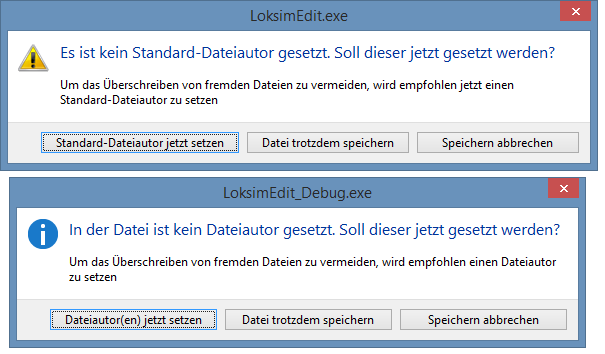
\includegraphics[width=1.0\textwidth]{editor/images/datei_ueberschreiben_empty.png}
\caption{Fehlermeldungen beim Speichern von Dateien ohne eingetragenem Standardersteller (oben) bzw. ohne eingetragenem Dateiautor (unten)}
\label{fig:editor-datei-ueberschreiben-empty}
\end{figure}

\begin{figure}
\centering
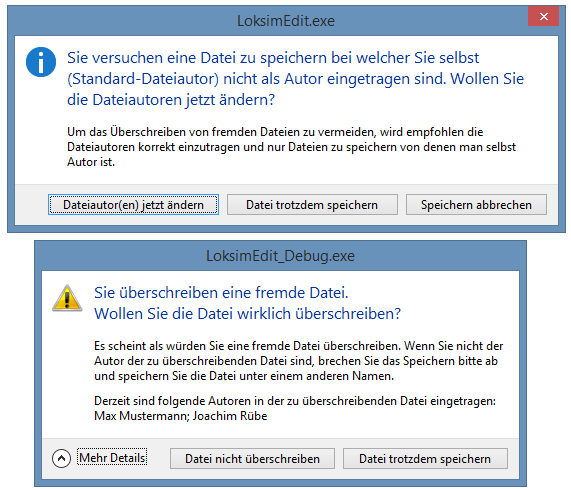
\includegraphics[width=1.0\textwidth]{editor/images/datei_ueberschreiben_overwrite.png}
\caption{Fehlermeldungen beim Speichern von Dateien bei denen man nicht selbst Dateiautor ist (oben) bzw. beim Überschreiben von fremden Dateien (unten)}
\label{fig:editor-datei-ueberschreiben-overwrite}
\end{figure}

Diese Lösung bietet keinen vollständigen Schutz vor dem Überschreiben fremder Dateien und schützt klarerweise überhaupt nicht vor dem Überschreiben von Dateien außerhalb des LoksimEdit. Ein vollständiger Schutz vor unbeabsichtigten Änderungen wäre wünschenswert, ist jedoch bei dem offenen Konzept von Loksim nicht einfach umzusetzen. Allerdings sollten die in Version 2.9 eingeführten Warnungen zumindest einen Teil der unabsichtlichen Änderungen verhindern.
\section{Package erzeugen}
\label{sec:editor.allg.packages}

Ein Package kann über das Menü Datei - Package erzeugen... erstellt werden.

Wird beim Suchen der abhängigen Dateien erkannt, dass eine Datei fehlt wird am Ende des Vorgangs eine Liste mit den fehlenden Dateien gezeigt.\abversion{2.9}

\subsection{Diese Dateien löschen / Packages deinstallieren}

Über die Schaltfläche Datei / Package hinzufügen lassen sich Dateien
hinzufügen, die bei der Installation des Package gelöscht werden sollen.
Hierbei ist es wichtig, dass nur Dateien hinzugefügt werden dürfen, die
sicher nicht von anderen Packages benutzt werden.

Seit Version 2.8.2 können auch ganze Packages hinzugefügt werden. Wird
ein Package hinzugefügt, wird dieses Package beim Benutzer
deinstalliert. Die Identifikation des Package erfolgt dabei über eine
Prüfsumme und nicht über den Dateinamen des Package. Ändert man etwas am
Inhalt des Package, ändert sich auch dessen Prüfsumme.

Es wird empfohlen bei neuen Versionen einer Strecke oder Führerstand die
alten Versionen des Package in diese Package deinstallieren Liste
hinzuzufügen. So werden beim Benutzer stets die nicht mehr benötigten
Dateien gelöscht

\section{Automatische Sicherung von Dateien}
\label{sec:editor-lastwork}
Der Editor speichert regelmäßig Sicherungskopien der gerade bearbeiteten Datei(en) im \emph{LastWork} Ordner im Datenverzeichnis. Dies ist nützlich falls man eine Änderung nach ein paar Tagen rückgängig machen möchte oder eine Datei unabsichtlich gelöscht hat.

Diese Sicherungsdaten werden auch für die Integration des sogenannten Restart Manager von Windows verwendet. Dies ermöglicht es nach einem etwaigen Absturz des LoksimEdit die zuletzt geänderten Dateien automatisch zu öffnen. Außerdem wird diese Funktion bei Neustarts des LoksimEdit bzw. von Windows verwendet (zB bei Installation einer neuen Loksim-Version oder bei Windows Updates).\abversion{2.9.3}

\emph{Hinweis:} Wir empfehlen Addon-Bauern trotzdem unbedingt eine regelmäßige Sicherung des Datenverzeichnis und das Aufheben von mehreren (älteren) Versionsständen. 
\section{Logging}\abversion{2.9.2}
\label{sec:editor-logging}

Im Verzeichnis \emph{\%LOCALAPPDATA\%/Loksim3D} werden für Loksim3D und für den LoksimEdit Logs erstellt. Diese umfassen derzeit noch wenige Informationen, werden aber in Zukunft mehr Daten enthalten.

In erster Linie können diese Logs für die Behebung von Fehlern genutzt werden und sie werden deshalb automatisch bei Fehlerberichten mitgesendet. Für Addon-Entwickler ergibt sich jedoch auch die Möglichkeit durch diese Logs (zusätzliche) Fehlermeldungen für die eigenen Addons mitzubekommen. Inbesondere in der Simulation können aus diversen Gründen nicht alle Fehlermeldungen (zB bzgl. fehlenden Dateien) angezeigt werden, wir bemühen uns diese in Zukunft zumindest in den Logs sichtbar zu machen.

\part{Anhang}
\chapter{Versionshistorie}
\section{Version 2.9.5}
\subsection{Neue Funktionen}
\begin{itemize}
\end{itemize}


\subsection{Kleinere Änderungen}
\begin{itemize}
\end{itemize}


\subsection{Fehlerkorrekturen}
\begin{itemize}
\item Editor: Standard Dateiinfo und -autor wird nun bei jedem Dateityp korrekt übernommen
\end{itemize}

\section{Version 2.10.1}\hfill 21. Dezember 2020

\subsection{Kleinere Änderungen}
\begin{itemize}
    \item LoksimEdit: Horiz. Zeiger (neu) ist Standard für neue Führerstände
    \item LoksimEdit: AFB Arten Wabco, Deuta und Wabco+Bremse als veraltet deklariert
    \item LoksimEdit: Drag-Geste für Schiene- und FontViews
\end{itemize}

\subsection{Fehlerkorrekturen}
\begin{itemize}
    \item Bugfix Rotation Streckenobjekt (\href{https://www.loksimulatoren.de/forum/index.php?thread/8430-gedrehte-streckenobjekte-ab-dem-2-modul-in-der-kbs-unsichtbar/}{Link Fehlerbeschreibung})
    \item Simulator: Doppelte Fahrplaneinträge (\href{https://www.loksimulatoren.de/forum/index.php?thread/8441-fehler-ebula-doppelte-haltepunkte-und-geschwindigkeitsanzeige/}{Link Fehlerbeschreibung})
    \item Simulator: Fehler in der "dynamischen Bremssteuerung" gefixt. Beim Umbenennen eine Funktion nicht richtig benannt. (\href{https://www.loksimulatoren.de/forum/index.php?thread/8442-dynamische-bremse-br427-428/&postID=137094#post137094}{Link Fehlerbeschreibung})
    \item Simulator: Bugfix Störungen von signalgedeckten BÜs (\href{https://www.loksimulatoren.de/forum/index.php?thread/5771-probleme-mit-durch-hauptsignale-%C3%BCberwachten-b%C3%BC/&postID=137100#post137100}{Link Fehlerbeschreibung})
    \item Simulator: FahrplanDaten::NextHalt ignoriert Zugfolgestellen und Betriebshalts (\href{https://www.loksimulatoren.de/forum/index.php?thread/5768-zza-anzeigen-falsch-wenn-hp-nur-als-zugfolgestelle-gekennzeichnet-ist/}{Link Fehlerbeschreibung})
    \item LoksimEdit: Bugfix Automatische Übernahme von Werten im Gruppenobjekteditor (\href{https://www.loksimulatoren.de/forum/index.php?thread/8262-speichern-von-%C3%A4nderungen-in-gruppenobjekten/}{Link Fehlerbeschreibung})
    \item LoksimEdit: Bugfix Menüführung Punkte verschieben/zoomen (\href{https://www.loksimulatoren.de/forum/index.php?thread/8431-fehler-der-men%C3%BCf%C3%BChrung-beim-verschieben-zoomen-von-objekten-im-gruppenobjektedit/}{Link Fehlerbeschreibung})
    \item LoksimEdit: Bugfix Standardeinstellungen Signale, Limits, Haltepunkte (\href{https://www.loksimulatoren.de/forum/index.php?thread/8435-standard-einstellungen-bei-signalen-werden-auch-bei-abbruch-gesetzt/}{Link Fehlerbeschreibung})
    \item LoksimEdit: Bugfix löschen aller Gleise (\href{https://www.loksimulatoren.de/forum/index.php?thread/8434-fehler-bei-l%C3%B6schen-des-letzten-gleises-einer-strecke/}{Link Fehlerbeschreibung})
\end{itemize}

\section{Version 2.10}\hfill 26. Oktober 2020
\subsection{Neue Funktionen}
\begin{itemize}
    \item Loksim: RailDriver Integration
    \item LoksimEdit: Überarbeitung Führerstandseditor
    \item LoksimEdit: ''Grab Geste'' fuer KBS-, Strecke-, Objektbitmap- und Führerstandsbitmap-View
    \item LoksimEdit: Letzer Zustand laden im Create Package Dialog
\end{itemize}


\subsection{Kleinere Änderungen}
\begin{itemize}
    \item Verbesserte Berechnung der Bounding Box von 3D-Fonts
    \item Loksim: SEP um textEBuLa erweitert
    \item Loksim: Verbesserung der Fahrplandarstellung im Führerstand
    \item LoksimEdit: 2D-View aktualisiert sich wenn Objekte geändert werden
    \item LoksimEdit: Englische Übersetzung für (neue) Teile des LoksimEdit
    \item LoksimEdit: Sichtwinkel bei Update in KBS-, und Strecke-View wiederherstellen
    \item LoksimEdit: Im Führerstandeditor sind veraltete Optionen deaktiviert
    \item PackageManager: Option Transaktionen zu deaktivieren
\end{itemize}

\subsection{Fehlerkorrekturen}
\begin{itemize}
    \item Bugfix beim Auswerten des Alphakanal
    \item Simulator: Bugfix bei Indusi zusätzlich: Korrektur der Berechnung der Signalposition
    \item Simulator: Bugfix Fst-Überblendung im Stand
    \item Simulator: Crash beim Blättern im Fahrtenschreiber
	\item Simulator: Bugfix AFB Zielgeschwindigkeit verharrte nach LZB-Aufnahme bei 160, obwohl höhere Geschwindigkeit angewählt war.
    \item LoksimEdit: Bugfix (Crash) Speichern von Backups wenn Pfad nicht beschreibbar
\end{itemize}


\section{Version 2.9.6}\hfill 22. Oktober 2019
\subsection{Neue Funktionen}
\begin{itemize}
    \item LoksimEdit: Dateilizenz kann angegeben werden
    \item \hyperref[sec:editor.allg.packages.l3dmeta]{LoksimEdit: Beim Erzeugen von Packages werden .l3dmeta Dateien ausgewertet - kann zum Definieren der Lizenz von externen Dateien verwendet werden}
\end{itemize}

\subsection{Kleinere Änderungen}
\begin{itemize}
\item Simulator: Anzeige Auflösung Führerstand im Auswahldialog
\item LoksimEdit: Meldung wenn Datei-Speichern fehlschlägt
\end{itemize}

\subsection{Fehlerkorrekturen}
\begin{itemize}
\item LoksimEdit: Bugfix beim Bestimmen von Abhängigkeiten von externen Objektformaten beim Erzeugen von Packages
\end{itemize}


\section{Version 2.9.5}\hfill 23. September 2019
\subsection{Neue Funktionen}
\begin{itemize}
    \item Simulator Exchange Protocols (SEP)
\end{itemize}


\subsection{Kleinere Änderungen}
\begin{itemize}
\item Normalenvektoren haben immer Laenge 1
\item Verbessertes Transparenzhandling bei Verwendung externer Objektformate
\item Umstellung Compiler: Visual C++ 2019
\end{itemize}

\subsection{Fehlerkorrekturen}
\begin{itemize}
\item Editor: Standard Dateiinfo und -autor wird nun bei jedem Dateityp korrekt übernommen
\item Lagekorrektur der Flügelschienen an der einfachen Weiche
\item Bugfix Checkbox "Objekt in Sichtweite ändert Sichtbarkeit nicht", wenn Funktion in Signalen verwendet wird
\end{itemize}


\section{Version 2.9.4}\hfill 20. Juli 2018
\subsection{Neue Funktionen}
\begin{itemize}
\item Erweiterung der Joystick-Schnittstelle. Es sind mehr als ein Joystick möglich
\item Joysticksteuerung (Buttons) erweitert
\item Erweiterung der TCP-Schnittstelle, Zustand der LM55/70/85 wird gesondert übertragen
\end{itemize}


\subsection{Kleinere Änderungen}
\begin{itemize}
\item LM Befehl40 im TCP-Protokoll nachgerüstet
\item PZB90 Restriktiver Modus wird nun korrekt an TCP, OLE und Fahrtenschreiber gemeldet
\item Weichendarstellung verbessert
\item Abfrage der aktuellsten Loksim-Version über HTTPS anstatt HTTP
\item Objekteditor: Textkoordinaten für einen Punkt auf einer Fläche für alle Flächen verwenden
\item Objekteditor: Beim Drücken von <ALT> werden alle Texturkoordinaten auf einmal verschoben
\end{itemize}


\subsection{Fehlerkorrekturen}
\begin{itemize}
\item Kleiner Bugfix bei der DKW-Darstellung
\item Bugfix Package Erstellen: Abwählen von Dateien funktioniert wieder
\item Bugfix PZB90: LM85/70/55 leuchtet waehrend restriktiver 1000Hz Beeinflussung nicht mehr
\item Korrektur der Fahrplandarstellung
\end{itemize}


\section{Version 2.9.3}\hfill 1. Jänner 2017
\subsection{Neue Funktionen}
\begin{itemize}
\item Neue Optionen für \hyperref[sec:editor-gleise]{Gleise}: Keine 3D-Darstellung, senkrechte Normalenvektoren und neue Transparenzoptionen
\item \hyperref[sec:sim-optionen-special]{Fahrplanabhängige Sichtweite}
\item Editor: Objekteditor zeigt Fehler bei Flächen an
\item Editor: \hyperref[sec:sec:editor-lastwork]{Integration Restartmanager}
\item Editor: Neuer Package Erzeugen Dialog und erweiterte Package Informationen
\item Editor: Backup von noch nicht gespeicherten Dateien im LastWork Ordner
\item Editor: Neue Option \emph{Ordnerstruktur übernehmen} bei Texturen optimieren
\item Objekteditor: Neuer Dialog für Punkte zu Fläche hinzufügen
\item Fonteditor: Textur zoombar
\item Objekteditor: \hyperref[sec:editor-obj-l3dobj-normalen]{Normalenvektoren für runde Objekte berechnen}
\end{itemize}


\subsection{Kleinere Änderungen}
\begin{itemize}
\item FahrplanDaten::LastHalt auch in Sichtbarkeitsausdruecken verfügbar
\item \hyperref[sec:sim-optionen-paths]{paths.ini} kann nun auch <Registry> anstatt Pfad enthalten
\item Interne Umstelllung der Gleiserzeugung
\item Indusi I60 ueberwacht nach 1000Hz in Stellung O auf 95km/h (zuvor 85km/h)
\item Editor: Bessere Kennzeichnung von fehlerhaften Eingaben in einigen Dialogen
\item Editor: \hyperref[sec:sec:editor-lastwork]{LastWork Ordner} behält bis zu 500 Dateien auf und sichert auch nichtgespeicherte Dateien
\item Editor: Liste von Variablen im Objekteigenschaften-Dialog in Zwischenablage kopierbar
\item Streckeneditor: Löschen aller Objekte eines Gleis auf einmal möglich
\item Strecken- und KBS-Editor: Anzeige Positionsinformationen über Info-Button
\end{itemize}


\subsection{Fehlerkorrekturen}
\begin{itemize}
\item Absturz beim Laden von Objekten die Punkte oder Linien enthalten aus externen Formaten behoben
\item Abstürze bei .l3dobj Objekten mit nicht-planaren Flächen behoben
\item Verschwinden von Objekten in bestimmten Situationen behoben
\item Zulassen von sehr kleiner Streckenrotation
\item Bugfix Behandlung von relativen Pfaden in speziellen Fällen
\item Bugfix Sichtbarkeit große Objekte 
\item Simulator: Bei ausgeblendeten Kennziffern wird ein Limit am Hauptsignal dennoch aktiv
\item Simulator: Probleme bei LZB-Ende behoben
\item Strecken- und KBS-Editor: Absturz bei bestimmten GPAs behoben
\item Streckeneditor: Bugfix Eigenschaftsname mit Sonderzeichen (Eigenschaften Gruppenobjekte)
\item Streckeneditor: Absturz GPA behoben
\end{itemize}


\section{Version 2.9.2}\hfill 11. August 2015
\subsection{Neue Funktionen}
\begin{itemize}
\item Zufallsdrehung bei Objekten auf Strecke möglich
\item \hyperref[sec.editor.obj.logischeausdruecke]{Zeichenketten in logischen Ausdrücken}
\item \hyperref[sec:editor-texturnutzung-optimieren]{Editor: Neue Funktion ''Texturnutzung optimieren''}
\item Objekteditor: Neuer Dialog für Punkte zu Fläche hinzufügen
\end{itemize}

\subsection{Kleinere Änderungen}
\begin{itemize}
\item Indusi-Einstellung PZ80R wird automatisch auf PZB90 PZ80R umgestellt
\item Kommandozeilen-Argument /renderstats:1 zeigt Anzahl von DrawCalls und Triangles
\item Optimierung bei externen Objektmodellen wenn kein Alphakanal in der Textur verwendet wird
\item \hyperref[sec:editor-logging]{Standardmäßiges Erstellen von Logs}
\item Reihenfolge der Gleise bei Verwendung von verknüpften BÜs nicht mehr relevant
\item Editor: FilePicture wird bei Speichern-Unter kopiert
\item Editor: Dateien die über ''Doppelklick'' im LoksimEdit geöffnet werden, erscheinen in RecentFileList
\item Editor: Beleuchtung mehr an Simulation angenähert
\item Editor: Löschen in Baumansichten mittels ''Entf''
\item Gruppenobjekteditor: Auswahl nach dem Löschen eines Objekts verbessert
\item Fonteditor: Speichern-Unter bei Fonts überschreibt existierende Texturen nicht mehr
\item PackageManager: Anzeige von Fehlern bei ''Installation Rückgängig machen''
\end{itemize}


\subsection{Fehlerkorrekturen}
\begin{itemize}
\item Bugfixes bei Sichtbarkeitssteuerung
\item Bugfix Rotation Streckenobjekte

\item ObjektEditor: Verschwinden von Objekten in seltenen Fällen
\item ObjektEditor: Texturkoordinaten ''Rückseite einfügen''

\item Streckeneditor: Setzen von Inhalt bei Textfeldern ohne Name bzw. bei Textfeldern mit dynamischer Sichtbarkeit
\item Streckeneditor: BÜ bei welchem der Name Teil des Namens eines andere BÜs ist, kann nun auch im GUI angelegt werden
\end{itemize}

\section{Version 2.9.1}\hfill 11. Jänner 2015

\subsection{Neue Funktionen}
\begin{itemize}
\item Streckeneditor: (Landschafts)objekte können nach Position sortiert werden
\end{itemize}

\subsection{Kleinere Änderungen}
\begin{itemize}
\item Optimierung Option ''Alle Texturen beim Start laden''
\item Vergrößerung von Eingabefeldern im Editor: Neu-Dialog, Rail - Höhenwerte der Bettung, Strecke - Unterbrechung der Höhenlinie
\item Performanceverbesserungen Packageinstallation
\item Behandlung nicht planarer Flächen bei Objekten die bis inkl. Version 2.9 erstellt wurden so wie in Version 2.8.3
\item Anzeige MessageBox bei fehlendem Sound im Simulator deaktiviert

\item Streckeneditor: Laden von Objekten für 2D-Ansicht erfolgt im Hintergrund
\item Streckeneditor: Graphikobjekte bei Streckeneigenschaften (Indusi-Magnete, Tafeln, etc) können nun jedes unterstützte Graphikformat sein (nicht nur .l3dgrp)
\item Streckeneditor: Button ''Rollmaterial anzeigen'' in ''Rollmaterial ausblenden'' umbenannt

\item Kursbucheditor: Standardauswahl bei neuer Verbindung im KBS-Editor optimiert
\end{itemize}

\subsection{Fehlerkorrekturen}
\begin{itemize}
\item ''Höhe über Landschaft'' bei global gesetzter Verschiebung in Y-Richtung
\item Gleichzeitiger Einsatz von ''Objekt mitdrehen'' und ''Zoomfaktor''
\item Texteigenschaft bei bestimmten Fonts
\item Streckenobjekte an Achse wiederholen und Verschiebung von Objekten
\item Einlesen ''2. Länge'' bei diversen Instrumenten von alten Führerständen

\item Editor: Mehrere 3D-Fenster gleichzeitig bedienen
\item Editor: Gehe-Zu-Postion Dialog aktualisiert 3D-Ansicht nicht
\item Editor: Bugfix Neu-Dialog bei geöffneter 3D-Ansicht
\item Editor: Korrektur Anzeige fehlender Dateien beim Erstellen von Packages
\item Editor: Bugfix Erstellen eines Package (Versionsinfo, zu löschende Dateien und Packages)

\item Objekteditor: Größenänderung Textur wird bei Drücken von ''Übernehmen'' Button erkannt
\item Objekteditor: Flächen kopieren

\item Gruppenobjekteditor: Nicht gesetzte Eigenschaft wird standardmäßig zu Wahr ''ausgewertet''
\item Gruppenobjekteditor: Objekte auf/ab
\item Gruppenobjekteditor: Punkte verschieben/zoomen Fonts

\item Streckeneditor: ''HelligkeitProzent'' nicht von manuell eingestellter Helligkeit beeinflusst
\item Streckeneditor: Erweiterte Objekteigenschaften bei Signalen
\item Streckeneditor: Einstellen von Eigenschaften verschachtelter Gruppenobjekte

\item Führerstandseditor: Undo/Redo
\end{itemize}


\section{Version 2.9}\hfill 9. November 2014

\subsection{Neue Funktionen}
\begin{itemize}
\item \hyperref[sec:editor-obj-grp]{Gruppenobjekte können selbst Gruppenobjekte enthalten}
\item \hyperref[sec:editor-obj-externe]{Unterstützung externer 3D-Objektmodellformate}
\item Möglichkeit \hyperref[sec:editor-strecke-obj-achsewiederholung]{Objekte auf Strecke an beliebiger Achse zu wiederholen}
% \item \hyperref[sec:editor-obj-textur-kachel]{Gekachelte Texturen bei Objekten}
\item \hyperref[sec:editor-obj-l3dobj-normalen]{Möglichkeit bei Objekten Normalenvektoren pro Fläche und nicht pro Punkt zu definieren}
\item Funktion \hyperref[sec:editor-obj-l3dobj-normalen]{''Berechnung Normalenvektoren''}
\item Funktion ''\hyperref[sec:editor-obj-grp-verschieben]{Gruppenobjekt}/\hyperref[sec:editor-obj-l3dobj-punkteverschieben]{Objekt} am Nullpunkt zentrieren''
\item \hyperref[sec:editor-obj-l3dobj-flaeche]{Funktion ''Rückseite einer Fläche automatisch erstellen''}
\item \hyperref[sec:editor-obj-sichtbarkeitssteuerung]{Überarbeitung und Erweiterung der Sichtbarkeitssteuerung}
\item \hyperref[sec:editor-allg-dateienueberschreiben]{Warnung beim Überschreiben fremder Dateien}
\item Neue Funktion \emph{Dateiabhängigkeiten anzeigen} im Expertenmodus des PackageManager verfügbar
\item \hyperref[sec:editor-obj-externe-konvertieren]{Konvertieren externer 3D-Objektmodellformate ins Loksim-Format}
\end{itemize}

\subsection{Kleinere Änderungen}
\begin{itemize}
\item Neue Systemvoraussetzung Windows Vista SP2 oder neuer 
\item \hyperref[sec:editor-obj-sichtbarkeitssteuerung-streig]{Möglichkeit Streckenmeter als Objekteigenschaft zu benutzen}
\item \hyperref[sec:editor-obj-logischeausdruecke-vars]{Variablen FahrplanDaten::Halt, BedarfshaltBahnsteig und BedarfshaltZug hinzugefügt}
\item \hyperref[sec:editor-obj-dynstr]{Neuer Operand FahrplanDaten::LastHalt für dynamische Schriften}
\item \hyperref[sec:editor-obj-dynstr-params]{Parameter von dynamischen Schriften können im Streckeneditor gesetzt werden}
\item Objektflächen müssen nicht konvex sein
\item Performanceverbesserungen
\item Objekte tauchen nicht mehr so plötzlich aus dem Nichts auf
\item \hyperref[sec:editor.allg.packages]{Fehlende Dateien beim Erstellen eines Package werden angezeigt}
\item Dialog Beleuchtung: ''Slider'' auf ''SpinBox'' geändert
\item Wegfall der Option \emph{Graphik unter x fps vereinfachen}
\item Neue Expertenoption zur Steuerung der \hyperref[sec.sim.optionen.darstellung]{Objektsichtweiten}
\item Neue Option \hyperref[sec.sim.optionen.darstellung]{Windows 8 Vollbildmodus}
\end{itemize}

\subsection{Fehlerkorrekturen}
\begin{itemize}
\item AFB ohne LZB-Führung nur bis 160 stellbar
\item Korrektur falsche Befreiungsmöglichkeit PZB90 1000Hz Beeinflussung
\item Zugsicherung Fahrsperre: Überwachungsgeschwindigkeit 2000Hz von 40km/h auf 10km/h verändert
\item Probleme Nachtführerstand und Standardgleis behoben
\item Korrektur OLE-Variable Wechselblinken
\item Fehler im PackageManager bei Deinstallation von Packages behoben
\item PZB-Befehl über Joystick wieder möglich
\item Editieren von Instrument Weglängenmessung korrigiert
\item Fehler beim Abspeichern benutzerdefinierter Charakteristik der Fahrstufen korrigiert
\end{itemize}

\section{Version 2.8.3}\hfill 2. April 2014

\subsection{Neue Funktionen}
\begin{itemize}
\item \hyperref[sec:editor-obj-transparenz]{Transparenz aus Alphakanal}
\item \hyperref[sec.sim.steuerung.diverses.wegmessung]{Zuglängenzähler}
\item \hyperref[paragraph.editor.gleis.gleiseigenschaften.signal.optiongruppensignal] {Signal - Option Gruppensignal}
\item \hyperref[subsubsec.editor.gleis.gleiseigenschaften.signaloptionen]{Signaloptionen - gleisabhängiges Zusatzsignal}
\item \hyperref[sec.editor.obj.logischeausdruecke]{Sichtbarkeitssteuerung - Variable VsigKennzahlKleiner}
\item \hyperref[sect.editor.lok.fst]{Nachtführerstandsbild}
\end{itemize}

\subsection{Kleinere Änderungen}
\begin{itemize}
\item Störschalter für PZB90
\item Verbesserung Verhalten PZB90 während LZB-Betrieb
\item Wegfall des 16px Rands für transparente \hyperref[sec:editor-obj-textur]{Texturen}
\item Dialog für den Aufruf der Hilfedateien
\item Erweiterung des Fahrtenschreibers um PZB-Tasten und LZB-Status
\item Anpassung der Uhrzeit-Werte im TCP-Protokoll an die Zusi2-Ausgaben (IDs 10, 11, 12, 50)
\item Digitale Instrumente können rechtsbündig dargestellt werden
\item Bei fehlender Fahrplandarstellung wird der erfolgreiche Halt im Buchfahrplan/EBuLa angezeigt
\item Unverriegelte Türen öffnen bei jedem Halt (auch auf freier Strecke) automatisch 
\end{itemize}

\subsection{Fehlerkorrekturen}
\begin{itemize}
\item Sound Ende 500Hz Überwachung
\item Fehlerkorrektur bei Überlagerung zweier 1000Hz Beeinflussungen (PZB90)
\item Korrekturen bei G- und S-Melder im LZB-Betrieb
\item Problem bei gleisabhängiger Sichtbarkeitssteuerung behoben
\end{itemize}

\section{Version 2.8.2a}\hfill 26. Juli 2013

\begin{itemize}
\itemsep1pt\parskip0pt\parsep0pt
\item
  Geschwindigkeiten über 160km/h mit LZB wieder möglich
\item
  Bedingtes Abspielen von Streckensounds
\end{itemize}

\section{Version 2.8.2}\hfill 18. Juli 2013

\begin{itemize}
\itemsep1pt\parskip0pt\parsep0pt
\item
  Bei der Darstellung des Buchfahrplans können die Spalten vier und fünf
  auf Rechtsbündig gesetzt werden.
\item
  Die Darstellung des Buchfahrplans kann auf EBuLa umgestellt werden.
  Die EBuLa-Anzeige ist nur vorbildähnlich.
\item
  2D-Fonts können sämtliche Zeichen aus Unicode enthalten
\item
  Gefahrene Km bzw. Anzahl Aufrufe werden auch pro Fahrplan gespeichert
\item
  Die Anzahl der Zeilen des Buchfahrplans im Führerstand kann nun im
  Editor gesetzt werden.
 \item 
  Komplette Neuimplementierung der PZB90
\item
  Stadtbahn PZB90  
\item
  Englische Version des Simulators
\item
  PackageManager: Deinstallation von Packages während Installation neuer
  Packages möglich
\item
  Joystick Achsen umkehrbar
\item
  Schneefall (Alpha Status) über Wetterdateien steuerbar
\end{itemize}

\begin{itemize}
\itemsep1pt\parskip0pt\parsep0pt
\item
  Der Indusimagnet des Schutzsignals wird eigenständig ausgewertet
\item
  Lüfter läuft nur bei Verwendung dynamischer Bremse nach
\item
  Lüfter schaltet mit HS aus
\item
  Anzeige Lüfterstatus verzögert anhand von Sound
\item
  Testen im LoksimEdit für Wetterdateien, Dynamische Schriften u.
  Dynamische Sichtbarkeitssteuerung verbessert
\item
  Kameraposition im (Gruppen)objekt-Editor bleibt nach Update-(Button)
  erhalten
\item
  Leerzeilen in der Buchfahplananzeige unterdrückt
\item
  Gruppenobjekt-Editor: Eigenschaften von Gruppenobjekt "überleben" ein
  Refresh der 3D-View
\item
  PackageManager: Anzeige von überschriebenen oder gelöschten
  schreibgeschützten Dateien ganz oben
\item
  Zufall pro Gruppenobjekt mit Sonstige::ZufallGruppenObjekt
\item
  CrashReport Sprache wird dynamisch anhand ausgewählter Sprache bei
  Installation bzw. PackageManager gesetzt
\item
  Sondersounds werden mit der Lautstärke für Ansagen abgespielt
\item
  Standard Sky-Datei wird nicht mehr automatisch im Fpl gesetzt
\item
  Darstellung Bedarfshalt in der Fpl-Anzeige geändert.
\item
  LoksimEdit: Datei-Öffnen Dialog enthält "Doku" Button
\item
  Verbesserte Auswahl für Standardauflösung und 3D-Treiber
\item
  Fette Überschriften im Lokeditor
\item
  Multimonitor-Support bei gleichen Treibernamen
\item
  TCP: Soll-Fahrstufe und Oberstrom
\end{itemize}

\begin{itemize}
\itemsep1pt\parskip0pt\parsep0pt
\item
  Bugfix Öffnen "Zuletzt verwendeter Datei" die nicht mehr existiert
\item
  PackageManager - Installation rückgängig machen bei schreibgeschützter
  Datei
\item
  Fehler bei Speichern unter - Textur kopieren behoben
\item
  Tippfehler und Texte im Lokeditor überarbeitet
\item
  'Verschleppte' Bezeichungen aus dem Nebengleis gefixed
\item
  Leerzeilen im Buchfahrplan Führerstand unterdrückt
\item
  Fehler in L3dEditLauncher behoben (mehrere Loksim Installationen)
\item
  Fehler in der Fahrplananzeige behoben
\item
  Mausradsteuerung
\item
  Verzerrter Sound im Stand
\item
  Korrektur Anzeige Bedarfshalt im Fst (manchmal zu früh)
\item
  Joystick mit Funktion "Kombibremshebel (inkl. Beschleunigung)" bei
  Fst. mit Kombibremshebeln verwendbar
\item
  Diverse Korrekturen bei LZB und AFB
\item
  Doppelter Nullstellzwang
\item
  Zs1 im LZB-Betrieb
\item
  AFB + Kombihebel
\end{itemize}

\paragraph{Version 2.8.1a}

07. Dezember 2012

\begin{itemize}
\itemsep1pt\parskip0pt\parsep0pt
\item
  Variable Sonstige::Zuglaenge
\item
  Senden der Daten in Fehlerberichten optimiert
\item
  Option Texturhandling standardmäßig auf "Bei Bedarf laden und nicht im
  Speicher halten"
\end{itemize}

\begin{itemize}
\itemsep1pt\parskip0pt\parsep0pt
\item
  AFB nur bis max. 160km/h ohne LZB
\item
  Bugfix Haltansagen
\item
  Bitmap bei "Font Erstellen" wird wieder automatisch generiert
\item
  PackageManager funktioniert auch auf FAT32 Partitionen
\item
  Kleinere Bugfixes im PackageManager
\end{itemize}

\paragraph{Version 2.8.1}

26. Oktober 2012

\begin{itemize}
\itemsep1pt\parskip0pt\parsep0pt
\item
  Die erste und zweite Spalte in der Fahrplandarstellungen der
  Führerstände sind jetzt als rechtsbündige Ausgabe möglich
\item
  Fonts sind jetzt wie Objekte über statische Zustandsvariablen
  schaltbar
\item
  Indusi zusätzlich: Nunmehr sind Geschwindigkeitsprüfabschnitte auch
  signalabhängig möglich
\item
  In Fahrplänen können benutzerdefinierte Variablen zur Verwendung in
  logischen Ausdrücken gesetzt werden
\item
  Trennung von Daten- und Programmverzeichnis möglich
\item
  Automatisches Erstellen von Fehlerberichten
\item
  Ein durchfahrener Halt kann als Zugfolgestelle definiert werden.
\item
  Ein Halt kann als Betriebshalt definiert werden.
\item
  Kachelung von Texturen in Skyboxen möglich
\item
  Texturen im PNG- und TGA-Format werden unterstützt
\item
  Dynamische Schriften möglich
\item
  LZB Verbesserungen: BKW und realistischere Bremskurven
\end{itemize}

\begin{itemize}
\itemsep1pt\parskip0pt\parsep0pt
\item
  Leuchtmelder Halbstufe reaktiviert
\item
  Steuerung S-Melder angepasst
\item
  Berechnung der Zuglänge im Bremszettel geändert
\item
  (Dis)connect Buttons für TCP-Anbindung eingebaut
\item
  PackageManager an kleinere Auflösungen angepasst
\item
  PackageManager kann installierte Dateien mit 'Doppelklick' sofort
  öffnen
\item
  Quadratische Texturen bei seitlichen Flächen in Skyboxen möglich und
  empfohlen
\item
  Bei Wetterauswahldialog ist standardmäßig "Zufällig" (Skybox)
  ausgewählt und nicht mehr die klassische Steuerung
\item
  Loksim(Edit) About-Dialog zeigt Verwendung von SSE2 an
\item
  Gebaeude1\_FFS von RainerH in Standard-Package 2.8.1 inkludiert
\item
  Anpassung an Benutzerkontensteuerung
\item
  Beim Package Erstellen kann man nun standardmäßig auch .txt, .pdf,
  .xps Dateien auswählen (Doku)
\item
  Über den Eigenschaften-Dialog kann man im LokimEdit jeder Datei eine
  Doku zuweisen. Für Fahrpläne und Loks wird im Loksim3D ein "Doku"
  Button zum Öffnen dieser Doku angezeigt
\item
  Joystick Slider (Schubregler) ist nutzbar
\item
  Bedarfshaltanzeiger kann im Editor mittels "Signal grün/rot" Button
  getestet werden
\item
  Bedarfshalt "immer" zu Testzwecken einstellbar
\item
  Zeitpunkt an dem Bedarfshalt-Anzeige im Fst aufleuchtet wird zufällig
  bestimmt
\item
  Installer regisistriert automatisch LoksimControl.exe
\item
  Speicherlimit für Loksim3D bzw. LoksimEdit auf 3 bzw. 4 GB angehoben
  (32 bzw. 64 Bit OS)
\item
  Erweiterung der logischen Ausdrücke

  \begin{itemize}
  \itemsep1pt\parskip0pt\parsep0pt
  \item
    FahrplanDaten::Ankunftszeit"\textless{}halt\textgreater{}"
  \item
    FahrplanDaten::Abfahrtszeit"\textless{}halt\textgreater{}"
  \item
    FahrplanVars::
  \item
    Funktionen::TimeDif(\textless{}arg1\textgreater{},
    \textless{}arg2\textgreater{})
  \end{itemize}
\item
  Neue Mausgesten bei der 3D Vorschau von Objekten
\item
  Normalenvektoren können im (Gruppen-)Objekteditor ausgeblendet werden
\item
  PreivewHandler zeigt Readme von .l3dpack Dateien
\item
  Joystickfunktionen Zugkraftregler (+/-) und AFB-Ziel (+/-) an
  Verhalten von Fahrstufe (+/-) angeglichen
\item
  Neue Icons
\end{itemize}

\begin{itemize}
\itemsep1pt\parskip0pt\parsep0pt
\item
  Vorsichtsignal (Zs7) ermöglicht ebenfalls die Abfahrt
\item
  Anzeige Indusi-Art in Fahrtenschreiber + LokInfo Anzeige korrigiert
\item
  Installer räumt Registry- und Startmenüeinträge bzw Dateien des alten
  Installers (2.7.2) auf
\item
  Abstürze des WetterEditors behoben
\item
  Streckensound im selben Ordner wie .l3dstr-Datei nun möglich
\item
  Ende Fahrt Anzeige überdeckt nicht mehr Fahrtauswertung
\item
  Diverse Tippfehler korrigiert
\item
  Bugfix für Anzeige Schnellbremsung bei OLE bzw. TCP
\item
  keine Soundkarte Fehlermeldung wird nur 1x gezeigt
\item
  Absturz LoksimEdit bei Verwendung von Touch-Monitor behoben
\item
  Fehler bei F11 bei kurzen Haltabständen behoben
\item
  Fehler bei Planabfahrt kurz nach 00:00 behoben
\end{itemize}

\paragraph{Version 2.8}

11. März 2012

\begin{itemize}
\itemsep1pt\parskip0pt\parsep0pt
\item
  Zusätzliche und erweiterte Signalfunktionen
\item
  Geschwindigkeitsprüfabschnitte
\item
  Logische Ausdrücke zur Sichtbarkeitssteuerung bzw Soundsteuerung
\item
  Wetter- / Himmelstextursteuerung
\item
  In Fahrplänen kann ein Sound definiert werden, welcher in einer
  bestimmten Entfernung vor einem (Bedarfs)halt abgespielt wird
\item
  Standarddateidialog auch unter Windows XP verwendbar
\item
  Neuer PackageManager für die (De)installation von Loksim-Packages
\item
  BÜ-Namen können nicht nur aus einer Liste ausgewählt werden, sondern
  auch direkt per Namen eingegeben werden (sinnvoll falls BÜ in anderer
  Streckendatei definiert ist)
\item
  Vertikaler Schriftzug bei Gruppenobjekten
\item
  Neue Hauptsignaleigenschaft als Checkbox: Zwischensignal
\item
  Einbau CH-Sifa mit und ohne HS-Auslösung. Minor Bugfixes CH-Indusi und
  neu Auslösung mit oder ohne HS-Auslösung.
\item
  Fehlende Verzögerung zwischen Schalten von BueLicht und BueSchranke
  bei Bahnübergängen eingebaut
\item
  {[}Vista+{]} Dateivorschau Handler (PreviewHandler) wird bei
  Installation registriert
\item
  {[}Vista+{]} Aufnahme der Loksim-Dateien in Windows-Suchindex bei
  Installation
\item
  Programmende beim Überfahren eines Rot zeigenden Signales ist
  abschaltbar
\item
  Erweiterung des Kombihbels um die Option "nur dyn. Bremse".
\item
  Fehlerkorrektur: Keine vZielüberwachung in der PZB bei Welchselblinken
  ohne 500er und 1000er-Melder.
\item
  Fehlerkorrektur: Nullstellungszwangauflösung über Zugkraft 0 möglich.
\item
  Joysticksteuerung bei Beschl+Bremsen mit Zugkraftregler korrigiert
\item
  Endlosschleifen KBS-Editor Weichenstellung verhindert
\item
  Bei der Zifferneingabe im Editor werden jetzt auch Kommas (Beistriche)
  akzeptiert
\item
  Real-Sifataste auch auf den Achsen der Joysticksteuerung
\item
  Bugfix beim Bestimmen des relativen Pfads von Loksim-Dateien gegenüber
  anderen Loksim-Dateien
\item
  Die Ausgabe 'Streckenlimit' so gesetzt, das auch ein Limit von 99km/h
  die Kennziffer 9 ergibt.
\item
  Standard-3D Einstellungen geändert: Max-Texturgröße 1024, Alle
  Texturen Laden und im Speicher halten, Hohe Farbtiefe, Cache nicht
  verwenden
\item
  L3dEditLauncher startet bei Vorhandensein mehrerer
  Loksim-Installationen immer den Editor im richtigen Ordner
\item
  Unterstützung von CrashDumps
\item
  Einsatz des SSE2 Befehlssatz bei neueren CPUs
\end{itemize}

\paragraph{Version 2.7.2}

12. Dezember 2010

\begin{itemize}
\itemsep1pt\parskip0pt\parsep0pt
\item
  Bug Lok Editor behoben (fehlende Eingabefelder für Instrumente)
\end{itemize}

\paragraph{Version 2.7.1}

29. November 2010

\begin{itemize}
\itemsep1pt\parskip0pt\parsep0pt
\item
  Erweiterte Bahnübergangssteuerung
\item
  Es kann der Sifa/Indusi-Zwangsbremsungssound mit der Option "nur
  einmal" versehen werden.
\item
  Auswertungs Bitmap funktioniert nun auch bei GDI Darstellung
\item
  Bug bei Laufleistung km Protokollierung behoben (alte Statistiken
  werden automatisch gelöscht)
\item
  Button Texturecache löschen funktioniert wieder
\item
  Streckensounds bei mehreren Modulen funktioniert nun
\item
  Bug in der Fahrtenschreiberauswertung behoben (- Prozente)
\item
  Bug bei Störungshäufigkeit von Signalgedeckten und Signalgedeckt
  (Streckenblock) BÜs
\item
  Standard Dateiinfo und -autor kann angegeben werden
\item
  Ab Vista kann anstatt dem loksimspezifischem der Standard Windows
  Dialog verwendet werden
\item
  Anzeige von Limits bei denen "Limit nicht anzeigen" gesetzt ist,
  werden standardmäßig in der EBULA nicht mehr angezeigt. Für Anfänger
  gibt es die Möglichkeit diese realitätssteigernde Option auszuschalten
\item
  Infofeld bei Fahrplan- und Lokauswahl vergrößert
\item
  Bug Haltestellenansage nach letztem Halt behoben
\item
  Bug Zs9 Meldung kommt nur mehr bei gestörten BÜs
\item
  PZB Befehl auf Maustaste möglich
\item
  Unnötige Änderungen übernehmen Nachfrage im Editor bei Weitsichtbar
  behoben
\item
  Streckensounds im Editor standardmäßig stummgeschaltet; Zustand der
  "Stummschaltung" wird bei Ein- und Ausschalten der Vorschau übernommen
\item
  Einbau SBB-Signum
\item
  Bug Uninstall behoben
\item
  Farbe und Breite für Sekundenzeiger in Analoguhr einstellbar
\item
  Bei Package-Installation werden die Zeitstempel bei versuchtem
  Überchreiben von schreibgeschützten Dateien angezeigt
\item
  Bug bei Zs1 behoben
\end{itemize}

\paragraph{Version 2.7}

1. Juli 2010

\begin{itemize}
\itemsep1pt\parskip0pt\parsep0pt
\item
  2D Darstellung standardmäßig mit DirectX
\item
  Möglichkeit Sounds auf Strecke einzubinden
\item
  Fehlerkorrekturen bei Packageinstallation
\end{itemize}



\end{document}
